\documentclass{article}

\usepackage{amsthm}
\usepackage{amsfonts}
\usepackage{amsmath}
\usepackage{amssymb}
\usepackage{fullpage}
\usepackage[usenames]{color}
\usepackage{hyperref}
  \hypersetup{
    colorlinks = true,
    urlcolor = blue,       % color of external links using \href
    linkcolor= blue,       % color of internal links 
    citecolor= blue,       % color of links to bibliography
    filecolor= blue,       % color of file links
    }
    
\usepackage{listings}
\usepackage{graphicx}
\graphicspath{ {./images/} }
\usepackage{mathtools}

\definecolor{dkgreen}{rgb}{0,0.6,0}
\definecolor{gray}{rgb}{0.5,0.5,0.5}
\definecolor{mauve}{rgb}{0.58,0,0.82}
\definecolor{mPurple}{rgb}{0.58,0,0.82}
\definecolor{mGreen}{rgb}{0,0.6,0}
\definecolor{red}{rgb}{1,0,0}

\lstdefinestyle{HaskellStyle}{
  frame=tb,
  language=haskell,
  aboveskip=3mm,
  belowskip=3mm,
  showstringspaces=false,
  columns=flexible,
  basicstyle={\small\ttfamily},
  numbers=none,
  numberstyle=\tiny\color{gray},
  keywordstyle=\color{blue},
  commentstyle=\color{dkgreen},
  stringstyle=\color{mauve},
  breaklines=true,
  breakatwhitespace=true,
  tabsize=3
}

\lstdefinestyle{CStyle}{
  frame=tb,
  language=C,
  aboveskip=3mm,
  belowskip=3mm,
  showstringspaces=false,
  columns=flexible,
  basicstyle={\small\ttfamily},
  numbers=none,
  numberstyle=\tiny\color{gray},
  keywordstyle=\color{blue},
  commentstyle=\color{red},
  stringstyle=\color{mauve},
  breaklines=true,
  breakatwhitespace=true,
  tabsize=3
}

\title{CPSC 353 Report}
\author{Scott Fitzpatrick  \\ Chapman University}

\date{\today}

\begin{document}

\maketitle

\begin{abstract}
The Haskell portion of this report is a kickstart guide for programmers with experience in imperative languages to learn functional programming, and more specifically, Haskell. From preparation of learning Haskell to the completion of a small Haskell program, this guide will be going over many of the basics in a follow-along fashion. There will be multiple small tasks which make up the entirety of the guide. It is meant to be unique in the aspect that it focuses on not only the general differences between imperative and functional programming, but also notes the syntax differences to avoid any confusion and frustration. Therefore, this guide is suitable for any programmers who are accustomed to programming in imperative languages and find functional programming to be less intuitive.
\end{abstract}

\tableofcontents

\section{Introduction}\label{intro}

First and foremost, this report will cover the programming language: Haskell. As stated in the abstract, Haskell will be examined in a kickstart guide format for programmers that are used to imperative programming languages.

\section{Haskell}\label{haskell}

\subsection{Preparation for Haskell}
\medskip\noindent
To learn and become familiar with Haskell, it is best that you prime yourself for success. I will share my opinions on the best ways to introduce yourself to Haskell.

\medskip\noindent
For installation of Haskell, see this page \href{https://hackmd.io/@alexhkurz/Hk86XnCzD}{this page}. It provides adequate information and links for installation. If lucky, this process should not take long. Keep in mind that if you are using Windows, it may be optimal to use \href{https://docs.microsoft.com/en-us/windows/wsl/install}{Windows Subsystem for Linux (WSL)} or \href{https://www.docker.com/get-started}{Docker}.

\medskip\noindent
It is also advantageous to use a good IDE that supports Haskell through plugins. I recommend \href{https://code.visualstudio.com/}{Visual Studio Code} with the \href{https://marketplace.visualstudio.com/items?itemName=justusadam.language-haskell}{Haskell Syntax Highlighting} plugin. It colorizes the code which makes viewing easier in all aspects. The syntax will be easier to get used to if you can consistently associate different colors with variables, functions, etc. I started without one of these plugins, and when the font is all white, things get confusing very quickly. \href{https://marketplace.visualstudio.com/items?itemName=Meowcolm024.has-go}{Haskell Runner} as another extension for Visual Studio Code that allows you to run haskell files within the IDE. However, I personally found that a classic terminal window works fine. You may also use other IDEs such as Emacs, Atom, or IntelliJ.

\medskip\noindent
Here is a trap to be weary of: assuming Haskell will be similar to other programming languages and that the process will feel familiar. This naive and costly mindset led me and some of my peers to fall behind after hitting unexpected and unfamiliar roadblocks. Be prepared to not only notice the differences in syntax, but rethink the functionality of code down to the core. Functional programming is much more theoretical and logic based. We will cover the details of this later. For now, it is best to prime yourself by preparing for completely new concepts that take mental flexibility to wrap your mind around. So be prepared to learn Haskell without any predispositions since things will seem somewhat different to imperative languages. It is also very important to pay close attention to the differences from imperative programming languages such as Python, Java, or C. For this tutorial, we will be comparing Haskell code with C.

\subsection{Introduction}
\medskip\noindent
My assumption is that you already know how to program in imperative languages such as C++, Python, or Java. Understanding how to code in these languages will make learning Haskell easier. However, it is important to make sure to prepare for the differences of functional programming.

\medskip\noindent
Functional Programming differences to prepare yourself for:
\begin{enumerate}
  \item One of these topics is the use of “pure” functions. These are bare-bone mathematical functions that your programs will function off of. Do not think of pure functions as instructions. Instead, think of them as definitions. It may be helpful to think of pure functions in Haskell similar to how you would think of actual mathematical functions such as those taught in school. Furthermore, pure functions do not have “side effects”. This means that evaluating an expression will not change some internal state which would later cause that same exact expression to have a different result. In a pure function, the same expression can be evaluated an infinite number of times and as long as the arguments are the same, the return value will stay the same.
  
  \item Immutable data is another aspect of functional programming. Similar to declaring a variable as a constant in an imperative language, Haskell variables will always be constant and you should not expect to mutate them. Though this may seem like a limitation, especially to an imperative programmer, immutables in Haskell have some advantages. Immutability in functional programming is essential for adopting a mathematical approach. This is because, in math, objects never change their state, and therefore requiring this immutability in programming will inadvertently make the code more mathematical. Immutable data can also be a major advantage when creating multithreaded applications. The consistency and immutability of variables is extremely useful for multithreaded applications because it prevents conflicts with different threads since variables do not change and the threads will use standard data. Of course, this aspect would be more relevant at an advanced level but it is something to keep in mind.
  
  \item Functional programming languages are declarative instead of imperative. Imperative programming uses a sequence of instructions on how to complete a task to obtain the result. On the other hand, in declarative programming the result is declared as the outcome of function applications. View this example:

  \begin{lstlisting}[style=HaskellStyle]
  -- HASKELL
  sum [] = 0
  sum (x:xs) = x + sum xs
  \end{lstlisting}

  \begin{lstlisting}[style=CStyle]
  // C CODE
  int sum(int *arr, int arrSize) {
    int i;
    int sum = 0;
  
    for (i = 0; i < arrSize; i++)
      sum += arr[i];
  
    return sum;
  }
  \end{lstlisting}

  Notice how in the imperative C code, there is explicit initialization of the variables and an explicit loop that will modify the data. These are explicit instructions for how to calculate the sum. Therefore it is imperative. On the contrary, the Haskell code, which is declarative, simply declares how the result is found with the use of addition and recursion. The second line of code is basically a mathematical function which contrasts with the C code, which is more like a series of instructions.

  \item Another key difference of functional programming that imperative programmers may not be used to is lazy evaluation. With lazy evaluation, expressions only get evaluated if they need to be. With imperative languages which are considered “strict”, an entire function can run, even if some of the computation is excessive and a waste of time and energy. Some functional programming languages such as Haskell will only compute what is needed to solve the task at hand. This is because evaluation is completely deferred until results are needed by other computations. This is obviously an advantage in the aspect that it can be much faster and efficient in certain scenarios. Also, since Haskell has these “non-strict” semantics, it allows for the processing of formally infinite data. 
\end{enumerate}

\subsection{Declecaring Variables with Types}
\medskip\noindent
Now that we have primed ourselves for learning Haskell, installed the proper software, and configured our IDE, we will begin with the basics such as types, functions, and more.Similar to imperative languages, when declaring variables in Haskell we must associate a type so that the computer knows what it is dealing with. 

\begin{lstlisting}[style=HaskellStyle]
-- HASKELL
x :: Integer
x = 1

y :: Bool
y = true

pi :: Float
pi = 3.1415
\end{lstlisting}

\begin{lstlisting}[style=CStyle]
// C CODE
int x;
x = 1;

bool y;
y = true;

float pi;
pi = 3.1415;
\end{lstlisting}

\medskip\noindent
At this point, the differences between Haskell and C are not too drastic, but be sure to note the differences in syntax and remember that the Haskell variables are immutable unlike the C variables.

\subsection{Defining a Function}
\medskip\noindent
To define a function follow the example:

\begin{lstlisting}[style=HaskellStyle]
-- HASKELL
out_of_range :: Integer -> Integer -> Integer -> Bool
out_of_range min max val = val < min || val > max
\end{lstlisting}

\begin{lstlisting}[style=CStyle]
// C CODE
bool out_of_range(int min, int max, int val) {
  if (val < min || x > max)
    return true;
  else
    return false;
}
\end{lstlisting}

\medskip\noindent
Similar to declaration variables with types, we must do the same with functions. The first line first states the name of the function followed by\verb| :: |. After this, the function parameter types are listed. In this case there are three integer types as the parameters that represent the min, max, and input value. The last type, which in this case is a boolean, is at the end. This may look confusing considering all of the types next to each other and separated with \verb|->|. It is important to remember that the last type is the return type and there can be as many input types as needed. Also using\verb| :: |between a function or variable name and its type can look strange at first but it is generally easy to get used to. In a way, it can be advantageous in the aspect that it stands out which is optimal when defining the type of a new variable.

\medskip\noindent
The second line actually defines how the function obtains the result. The function name followed by the input variable names are located on the left hand side of the equals sign. On the other side, the computation is made with the assistance of the less than and greater than operands (which are functions themselves). In this case, it simply checks if the value is below the minimum or above the maximum.

\medskip\noindent
Notice how this function declaration, when it comes down to it, is really a boolean value. This contrasts with the C function which is instructions to get this same value. This ties back to the aspect of declarative versus imperative programming.

\subsection{Calling a Function}
\medskip\noindent
Calling a function is rather simple. View this example:

\begin{lstlisting}[style=HaskellStyle]
-- HASKELL
result :: Bool
result = out_of_range 4 7 5
\end{lstlisting}

\begin{lstlisting}[style=CStyle]
// C CODE
bool result;
result = out_of_range(4, 7 ,5)
\end{lstlisting}

\medskip\noindent
The function is simply called by typing the name of the function followed by the inputs. In this particular example, we are assigning the result to a boolean variable for sample context. The result would be false. One syntax difference that may take some getting used to is the fact that there are no parentheses in Haskell like there usually is in imperative languages such as C in this example. I personally always associated functions and calling functions with parentheses, and when working with Haskell it took me a while to get used to seeing a function with its parameters simply listed out behind it with spaces. Furthermore, remember to use the right type as inputs to the function. If, for example, a float was used instead of an integer, it would create a type error.

\subsection{Function "let"}
\medskip\noindent
With Haskell, you may assign a value to a name, which can later be used to define the last expression or result. This can create more flexibility when programming with Haskell. Consider this example:

\begin{lstlisting}[style=HaskellStyle]
-- HASKELL
out_of_range :: Integer -> Integer -> Integer -> Bool
out_of_range minBound maxBound val =
  let out_of_lower_bound = minBound > val
      out_of_upper_bound = maxBound < val
  in
  out_of_lower_bound || out_of_upper_bound
\end{lstlisting}

\begin{lstlisting}[style=CStyle]
// C CODE
bool out_of_range(int minBound, int maxBound, int val) {
  bool out_of_lower_bound = minBound > val;
  bool out_of_upper_bound = maxBound < val;

  return out_of_lower_bound || out_of_upper_bound;
}
\end{lstlisting}

\medskip\noindent
Take your time observing the format of the syntax. The Haskell code is very similar to C in this instance. One of the biggest differences in terms of appearance is how the function declaration uses a \lstinline{let} and an “in” statement. With this format, Haskell let functions are still functional programming since the function is still equivalent to a boolean value. Unlike the C code, there were no step-by-step instructions that led to a return type.

\subsection{Function "where"}
\medskip\noindent
Similar to \verb|let|, \verb|where| allows you to use multiple variables with assigned values to define the function. However, \verb|where| does this after the initial function declaration. View this example:

\begin{lstlisting}[style=HaskellStyle]
-- HASKELL
out_of_range :: Integer -> Integer -> Integer -> Bool
out_of_range minBound maxBound val = out_of_lower_bound || out_of_upper_bound
  where
    out_of_lower_bound = minBound > val
    out_of_upper_bound = maxBound < val
\end{lstlisting}

\medskip\noindent
In my opinion, \verb|where| functions look much cleaner and readable than \verb|let| functions, but your choice is obviously up to you. Also, the corresponding C function would just be the same as the previous C example for \verb|let|.

\subsection{Using “if”, “else if”, “else”, and “then”}
\medskip\noindent
In Haskell you may also use \verb|if| and \verb|else if|, and \verb|else| statements. We will use them in the same function for convenience. View the example below:

\begin{lstlisting}[style=HaskellStyle]
-- HASKELL
out_of_range :: Integer -> Integer -> Integer -> Bool
out_of_range minBound maxBound val =
  if minBound > val then True
  else if maxBound < val then True
  else False
\end{lstlisting}

\begin{lstlisting}[style=CStyle]
// C CODE
bool out_of_range(int minBound, int maxBound, int val) {
  if (minBound > val)
    return true;
  else if (maxBound < val)
    return true;
  else 
    return false;
}
\end{lstlisting}

\medskip\noindent
If you saw, the statements are not too different from imperative C. However, they are followed by \verb|then| which precedes the resulting value of the function determined by the boolean statement. Also, keep in mind that in Haskell, \verb|True| and \verb|False| are capitalized unlike C.

\medskip\noindent
Furthermore, this can be simplified syntactically by using guards:

\begin{lstlisting}[style=HaskellStyle]
-- HASKELL
out_of_range :: Integer -> Integer -> Integer -> Bool
out_of_range minBound maxBound val
  | minBound > val then True
  | maxBound < val then True
  | otherwise False
\end{lstlisting}

\subsection{Recursion and Pattern Matching}
\medskip\noindent
In imperative languages it is routine to use loops in order to obtain results and calculations from whatever the computation may be. However, in Haskell loops do not exist. You may wonder, “How am I supposed to accomplish anything then?”. The answer is: recursion. If you are unfamiliar with recursion, it may be good to practice it in an imperative language first. \href{https://www.geeksforgeeks.org/c-program-for-fibonacci-numbers/}{Here} is an article on writing a recursive C program for Fiibonacci numbers. Remember that functions are recursive when they call themselves.

\medskip\noindent
For our example, we will also be doing a recursive Fibonacci function. We will explore pattern matching in this example too. View the Haskell sample below:

\begin{lstlisting}[style=HaskellStyle]
-- HASKELL
fib :: Integer -> Integer
fib 0 = 1
fib 1 = 1
fib n | n >= 2 = fib (n-1) + fib (n-2)
\end{lstlisting}

\medskip\noindent
You may be confused by the | symbol. However, it does not have any value and is just a separator. Also, the preceding second and third line: \verb|fib 0 = 1| and \verb|fib 1 = 1| may be confusing. This is where pattern matching comes into play. Pattern matching is like piecewise functions in math. For example, his would be the corresponding mathematical piecewise function for the Fibonacci function:

\begin{equation*}
fib(n)=\begin{cases}
          1, \quad &\text{if} \, n = 0 \\
          1, \quad &\text{if} \, n = 1 \\
          fib(n-1)+fib(n-2), \quad &\text{if} \, n \geq 2 \\
      \end{cases}
\end{equation*}

\medskip\noindent
When calling the function, the designated body is chosen with comparison of arguments. In this instance if n is 0 or 1, 1 is returned. If n is greater than or equal to 2, Fibonacci expressions are executed and the recursion commences. The first two rows of this piecewise function act as base cases and the same goes for the Haskell code on lines two and three. It may also be easier to compare this piecewise function with a syntactically simplified version of the Haskell Fibonacci function with “|” guards. Here is that version:

\begin{lstlisting}[style=HaskellStyle]
-- HASKELL
fib :: Integer -> Integer
fib n | n == 0 = 1
      | n == 1 = 1
      | n >= 2 = fib (n-1) + fib (n-2)
\end{lstlisting}

\medskip\noindent
Also, here is the imperative C code for the same function:

\begin{lstlisting}[style=CStyle]
// C CODE
int fib(int n) {
  if (n <= 1)
    return n;
  else
    return fib(n - 1) + fib(n - 2);
}
\end{lstlisting}

\section{Programming Languages Theory}

\subsection{Introduction to String Rewriting}

\medskip\noindent
Why Should One Study Abstract Reduction Systems?

\medskip\noindent
String Rewriting, and more specifically, String Reduction Systems (ARS) are significant because they can be instantiated at various levels of abstraction. This can be done in hardware with algorithms, programming languages, and high-level software engineering. ELABORATE. ARS's can be used to demonstrate and define properties such as normal forms, termination, and confluence.

\medskip\noindent
Though the term "abstract reduction systems" may sound fancy or intimidating, it is not too different from what is studied in math at a middle-school level. Just as mathematical algebra equations can be solved in a variety of ways to obtain the same result, ARS's do the same. Equational theory and rewrite systems are almost equivalent. The main difference is that ARS's are usually evaluated from left to right, unlike algebriac equations which can be evaluated in whichever direction.


\subsection{Brief Quickstart: What is an Abstract Reduction System (ARS)?}

\medskip\noindent
An ARS is a set of data paired with a set of rules. Oftentimes the data is referred to as objects. The set of rules define the binary relationship between objects. The notation appears as: (A, R) where A is the set of data and R is the set of rules. The binary relationship denoted by $\rightarrow$ and is called the reduction relation. ELABORATE ON DIFFERENT KINDS OF REDUCTION

\medskip\noindent
View this simple ARS example:

\begin{figure}[h!]
  \centering
  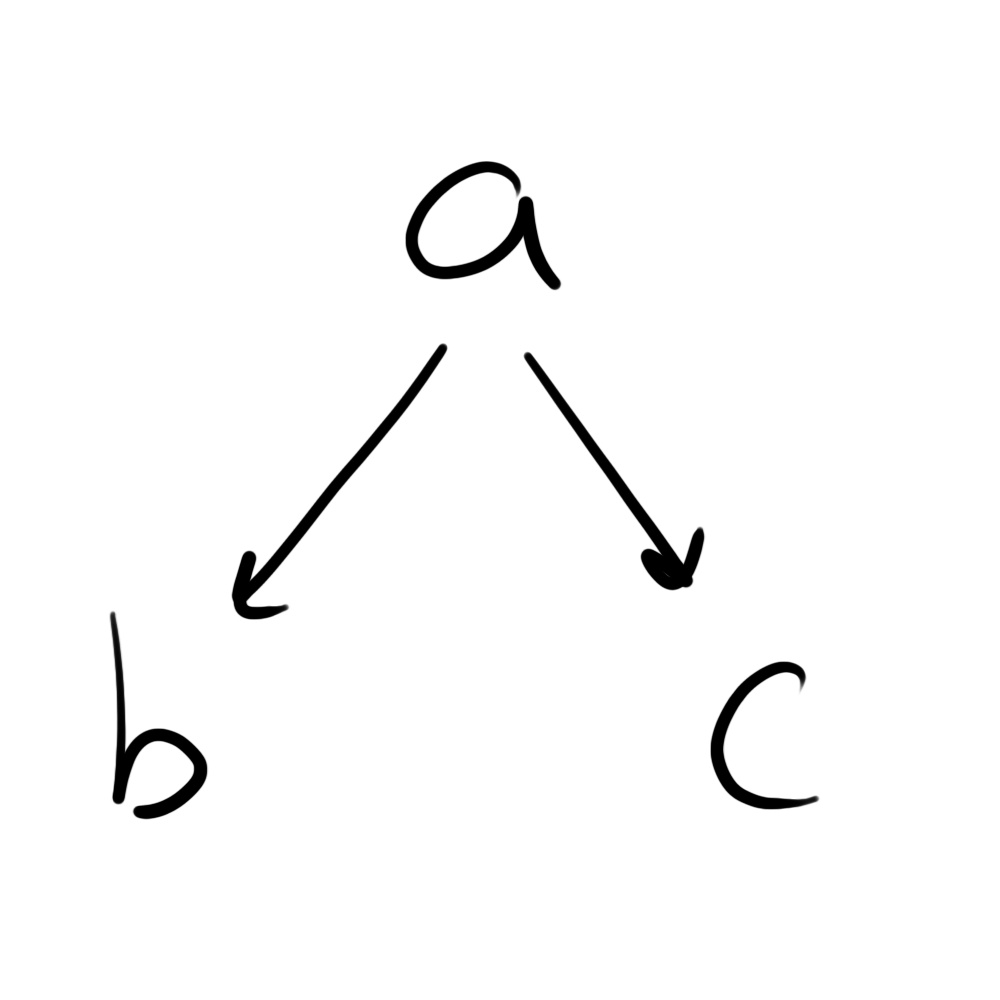
\includegraphics[scale=0.06]{gen1}
  \caption[] {
    \tabular[t]{@{}l@{}} ARS = (A, R) \\ A = \{a, b, c\} \\ R = \{(a, b), (a, c)\}
    \endtabular}
\end{figure}

\medskip\noindent
We obtain that our set of objects (A) consists of a, b, and c. From (a, b) and (a, c), we also see that our rules are that a $\rightarrow$ b and a $\rightarrow$ c. These rules define the binary relationship between a, b, and c.

\medskip\noindent
Here is another example of a simple ARS where A = \{a, b\} and R = {(a, b), (b, b)\}. The visual of this is:

\begin{figure}[h!]
  \centering
  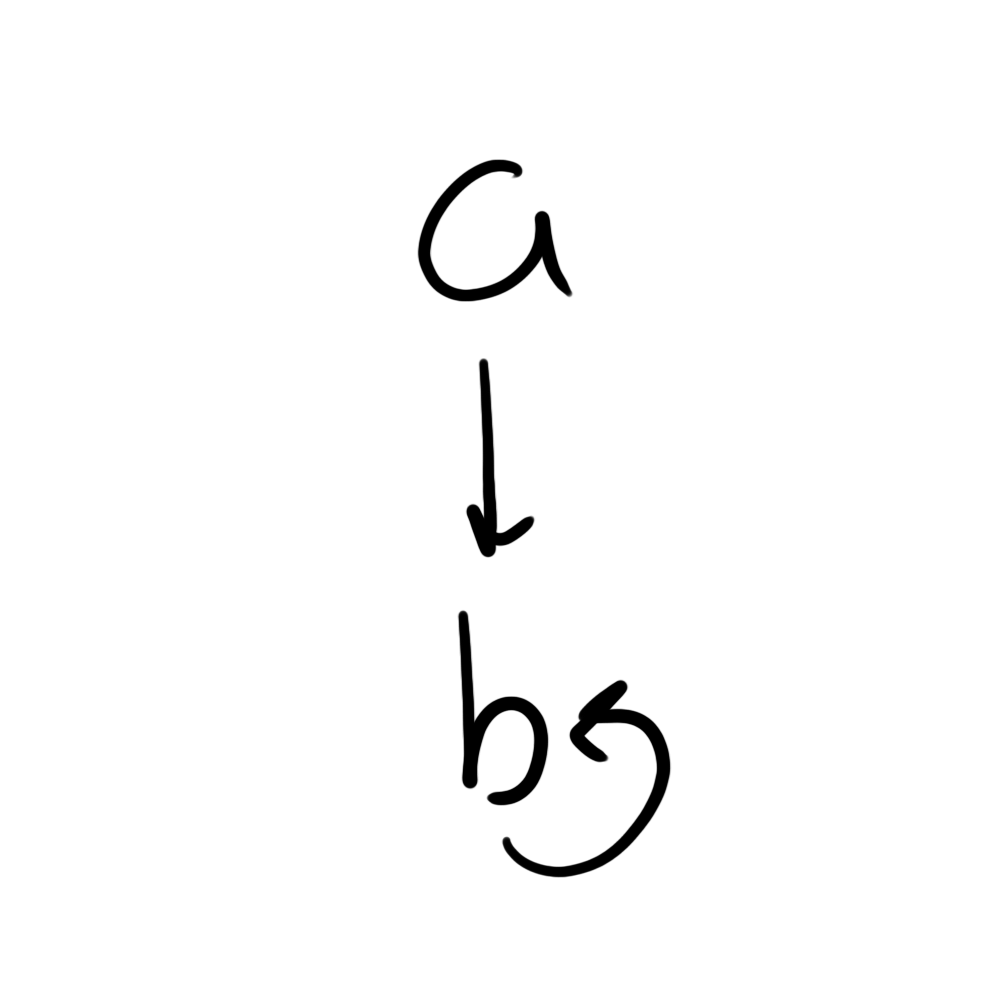
\includegraphics[scale=0.06]{gen2}
  \caption[] {
    \tabular[t]{@{}l@{}} ARS = (A, R) \\ A = \{a, b\} \\ R = \{(a, b), (b, b)\}
    \endtabular}
\end{figure}

\medskip\noindent
TALK ABOUT THE UNIQUENESS OF THIS ARS AND TRANSITION TO HOW THERE ARE INIFINITE POSSIBILITIES ALL WITH THEIR OWN SPECIAL PROPERTIES AND FEATURES

\medskip\noindent
There are infinite ARS examples that can be viewed for further exploration. For the purpose of keeping this quickstart brief, we will move on and view more specific examples.


\subsection{Significant Properties of Abstract Reduction Systems}

\subsubsection{Termination}

\medskip\noindent
From basic intuition you may have guessed that if an ARS is terminating, then it will always stop at some point when executed. If you have guessed this, then you are correct. When there are no loops in an ARS, it will eventually terminate. Here are some examples of terminating and non-terminating ARS’s.

\begin{figure}[h!]
  \centering
  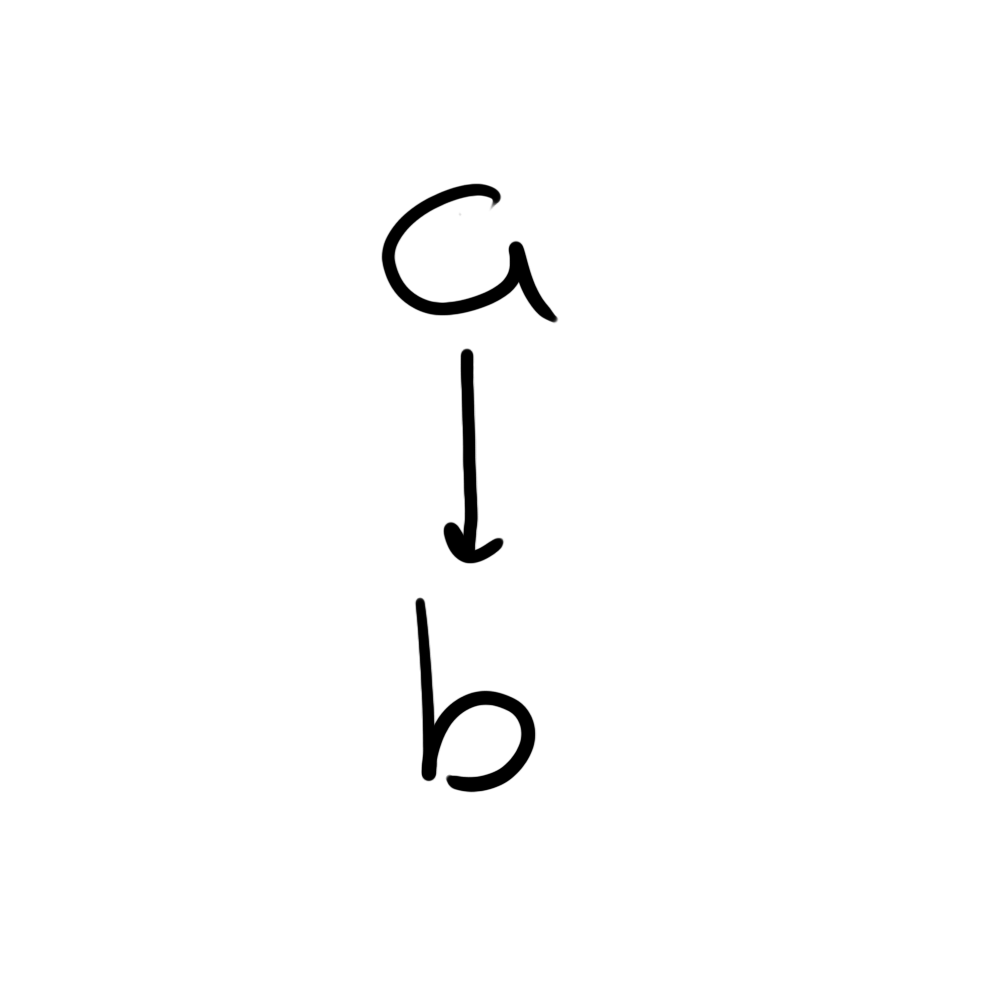
\includegraphics[scale=0.06]{gen3}
  \caption[] {
    \tabular[t]{@{}l@{}} ARS = (A, R) \\ A = \{a, b\} \\ R = \{(a, b)\}
    \endtabular}
\end{figure}

\begin{figure}[h!]
  \centering
  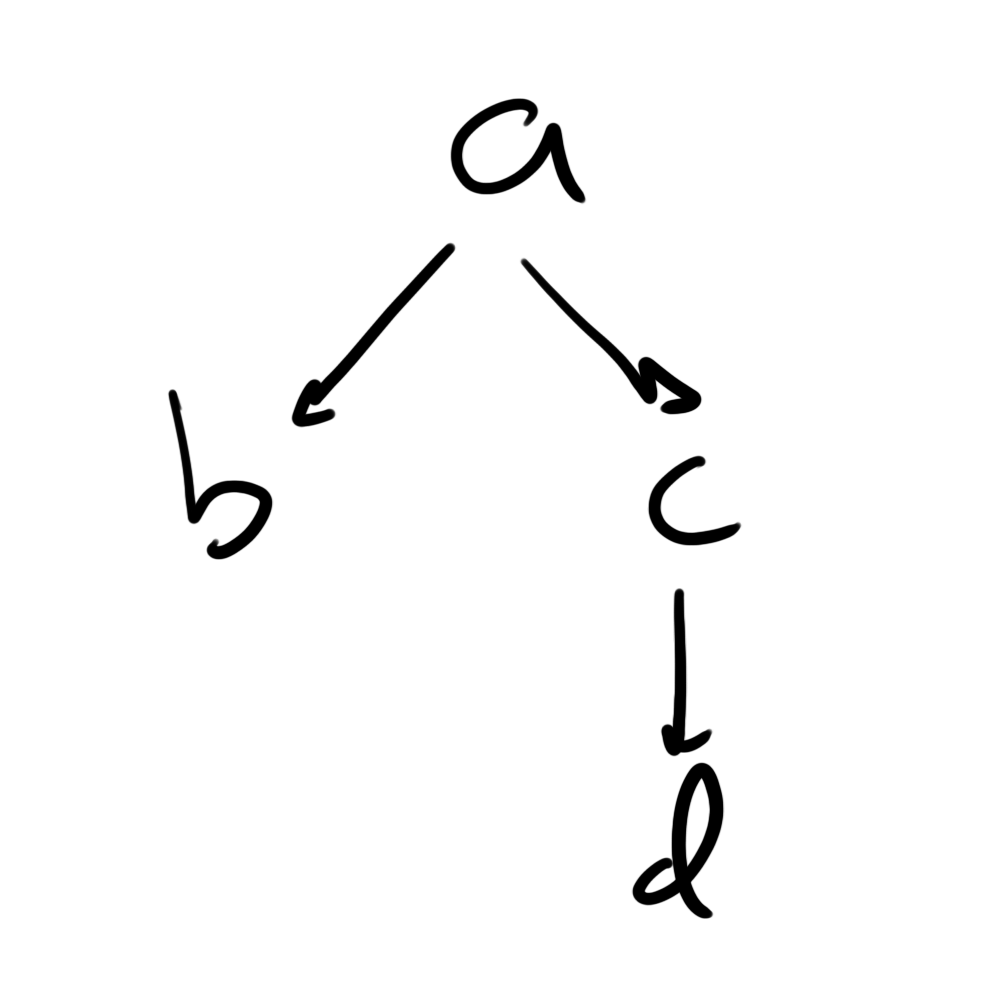
\includegraphics[scale=0.06]{gen4}
  \caption[] {
    \tabular[t]{@{}l@{}} ARS = (A, R) \\ A = \{a, b, c, d\} \\ R = \{(a, b), (a, c), (c,d)\}
    \endtabular}
\end{figure}

\begin{figure}[h!]
  \centering
  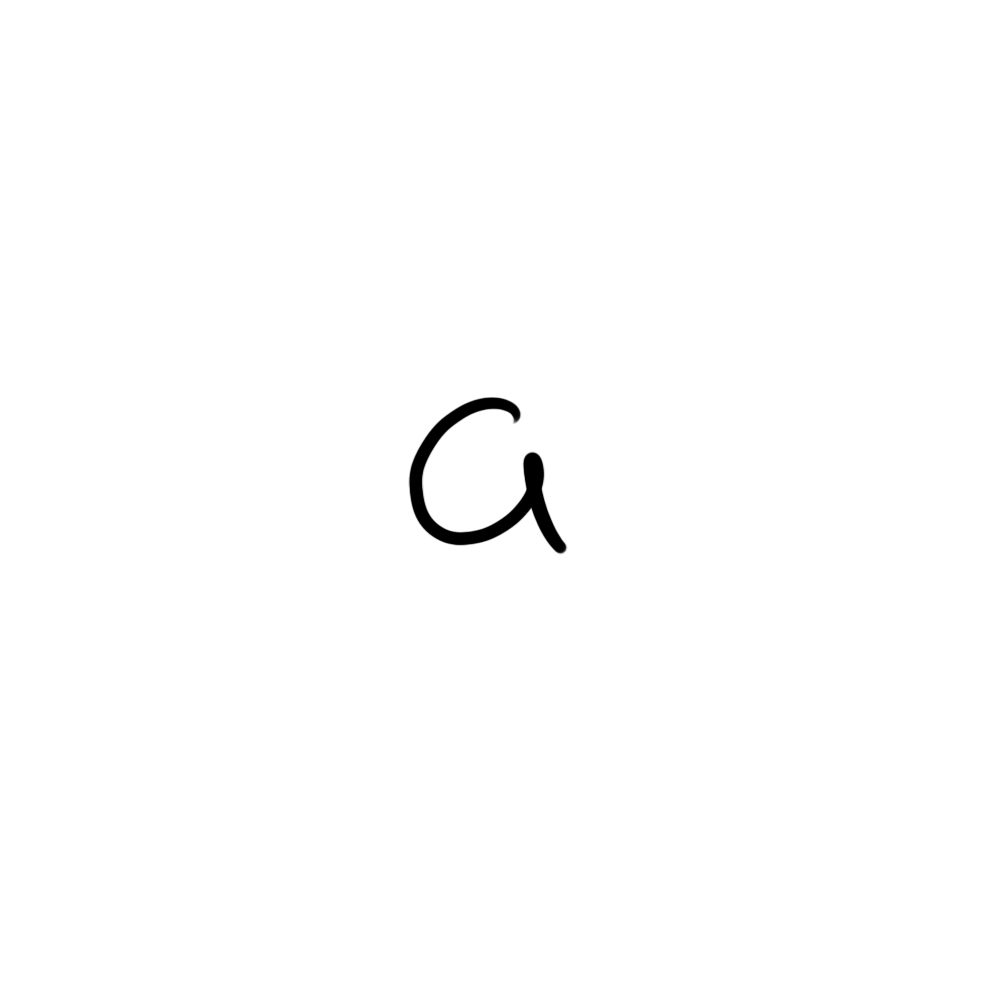
\includegraphics[scale=0.06]{gen5}
  \caption[] {
    \tabular[t]{@{}l@{}} ARS = (A, R) \\ A = \{a\} \\ R = \{\}
    \endtabular}
\end{figure}

\medskip\noindent
Note how in all of these examples above, the ARS reaches a definite end at some point. Therefore, it is terminating. Here are some examples of non-terminating ARS's. ELABORATE

\begin{figure}[h!]
  \centering
  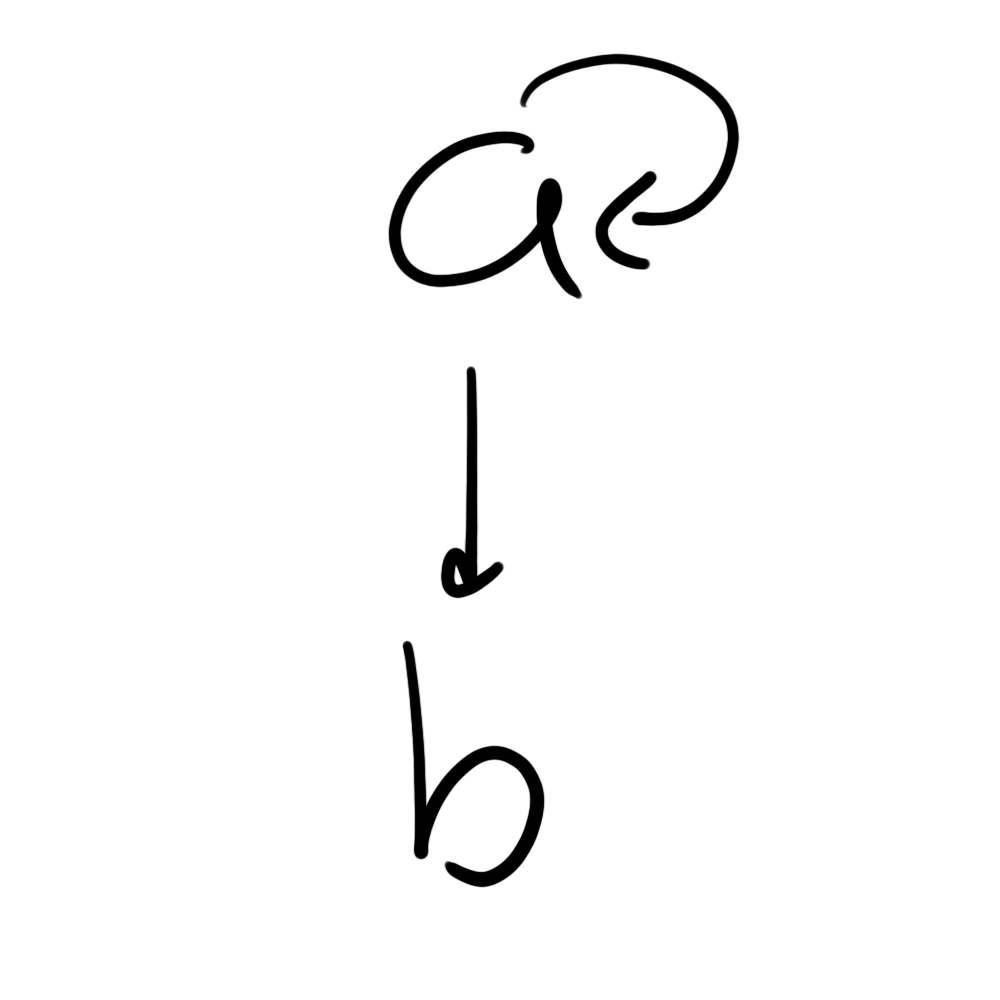
\includegraphics[scale=0.06]{gen6}
  \caption[] {
    \tabular[t]{@{}l@{}} ARS = (A, R) \\ A = \{a, b\} \\ R = \{(a, a), (a, b)\}
    \endtabular}
\end{figure}

\begin{figure}[h!]
  \centering
  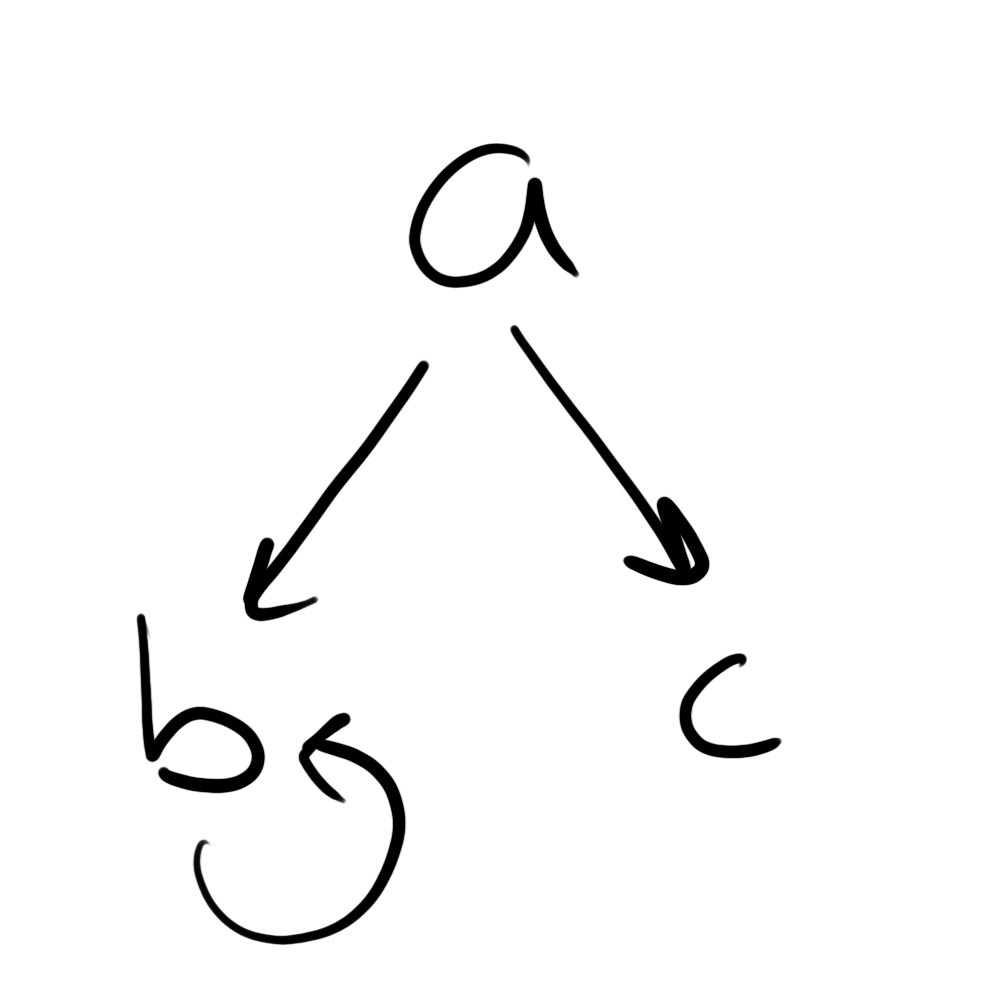
\includegraphics[scale=0.06]{gen7}
  \caption[] {
    \tabular[t]{@{}l@{}} ARS = (A, R) \\ A = \{a, b, c\} \\ R = \{(a, b), (b, b), (a, c)\}
    \endtabular}
\end{figure}

\begin{figure}[h!]
  \centering
  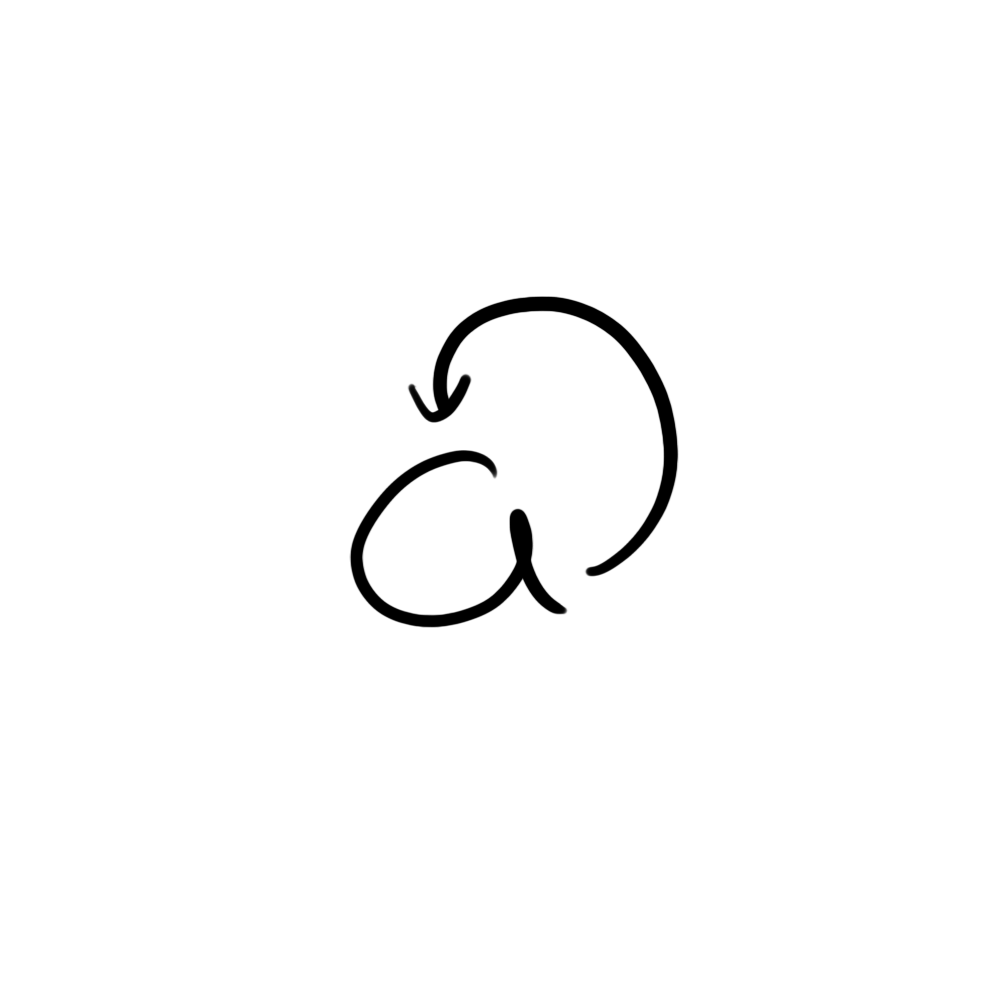
\includegraphics[scale=0.06]{gen8}
  \caption[] {
    \tabular[t]{@{}l@{}} ARS = (A, R) \\ A = \{a\} \\ R = \{a, a\}
    \endtabular}
\end{figure}

\medskip\noindent
Notice how in all of these examples there is a loop that prevents the ARS from completely terminating. Even if one path allows for termination, if there are any portions of the ARS where it could loop, the entire ARS is considered non-terminating. When an ARS has a loop, it is non-deterministic, meaning that it will not have the same result every time. ELABORATE


\subsubsection{Unique Normal Form (UNF)}

\medskip\noindent
To define a unique normal form, we must first define a normal form. A normal form is an object that no rules can apply to. This also implies that it is the end of the computation and can be recognized when there are no arrows stemming from the object. Here are some examples of normal forms:

\begin{figure}[h!]
  \centering
  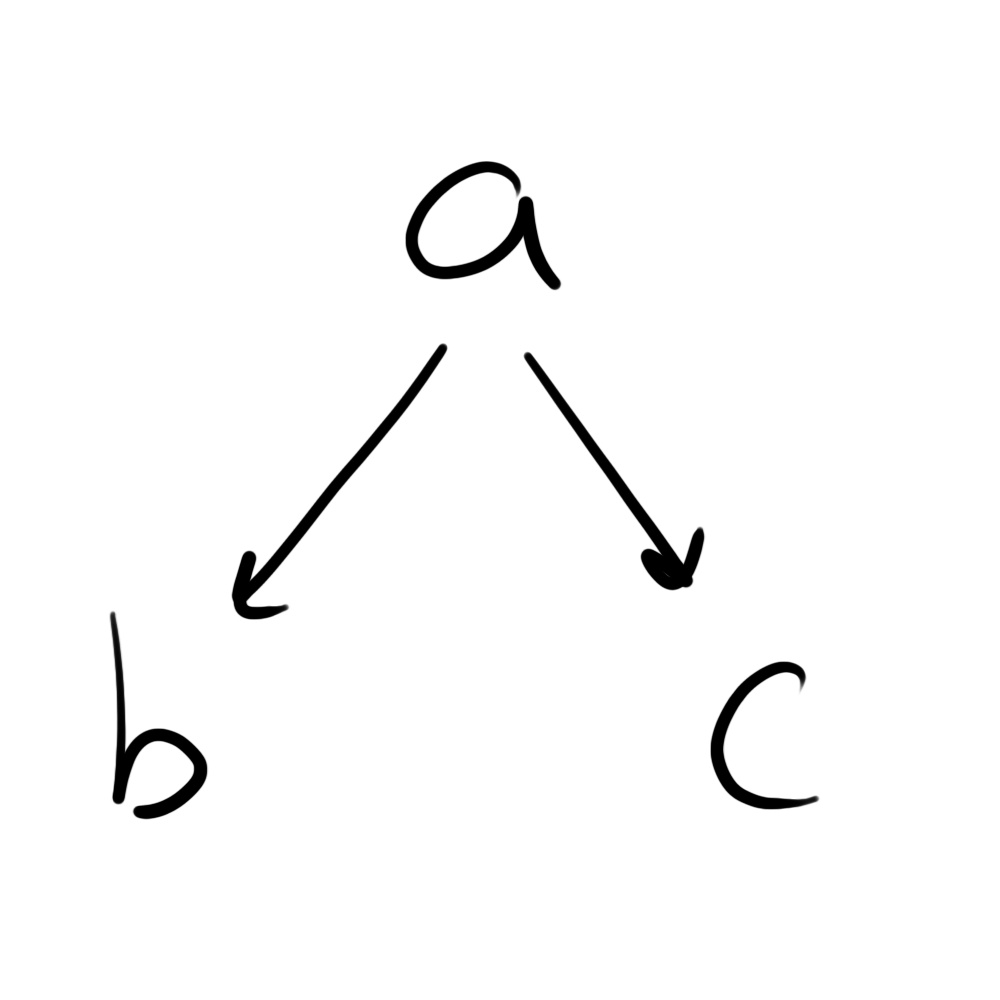
\includegraphics[scale=0.06]{gen9}
  \caption[] {
    \tabular[t]{@{}l@{}} ARS = (A, R) \\ A = \{a, b, c\} \\ R = \{(a, b), (a, c)\}
    \endtabular}
\end{figure}

\begin{figure}[h!]
  \centering
  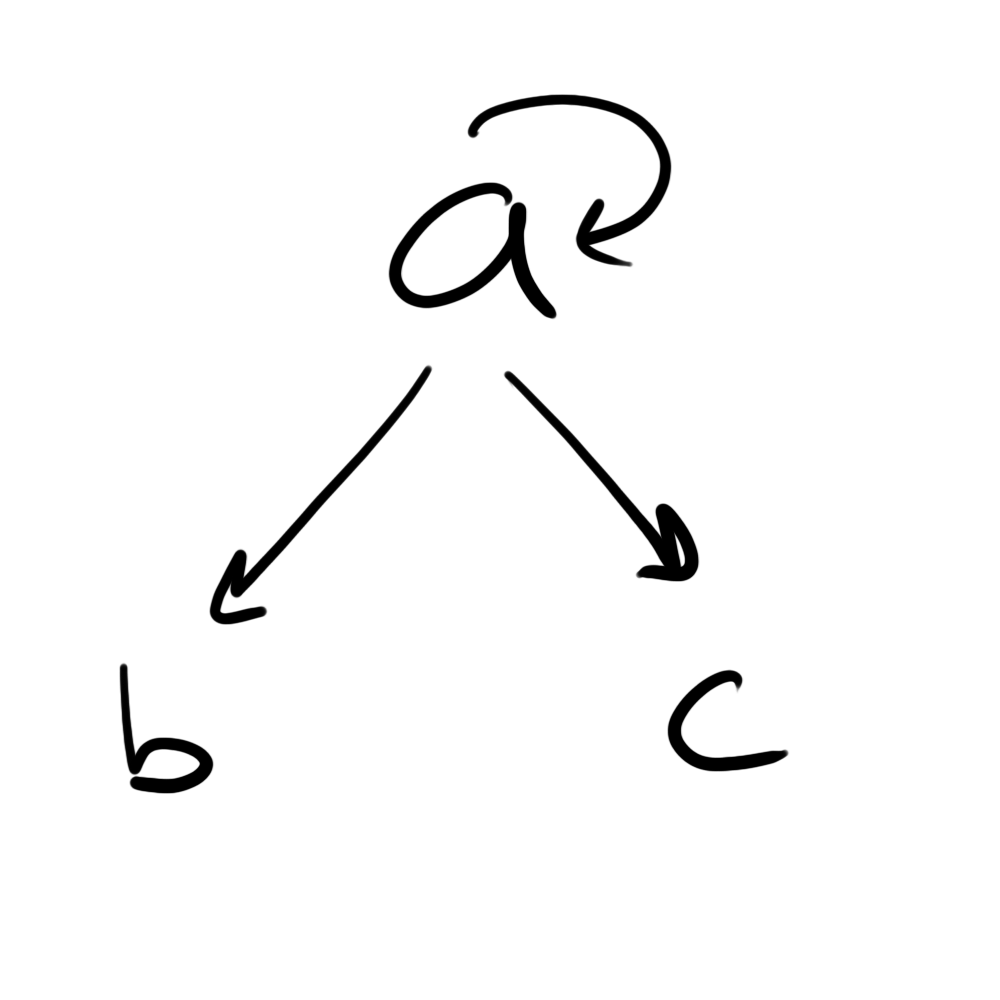
\includegraphics[scale=0.06]{gen10}
  \caption[] {
    \tabular[t]{@{}l@{}} ARS = (A, R) \\ A = \{a, b, c\} \\ R = \{(a, a), (a, b), (a, c)\}
    \endtabular}
\end{figure}

\medskip\noindent
A unique normal form (UNF) is the same thing, except it is the one and only normal form of the ARS. It is called the “unique” normal form because it is the only normal form that the ARS will result in. ELABORATE. Here are some examples of unique normal forms:

\begin{figure}[h!]
  \centering
  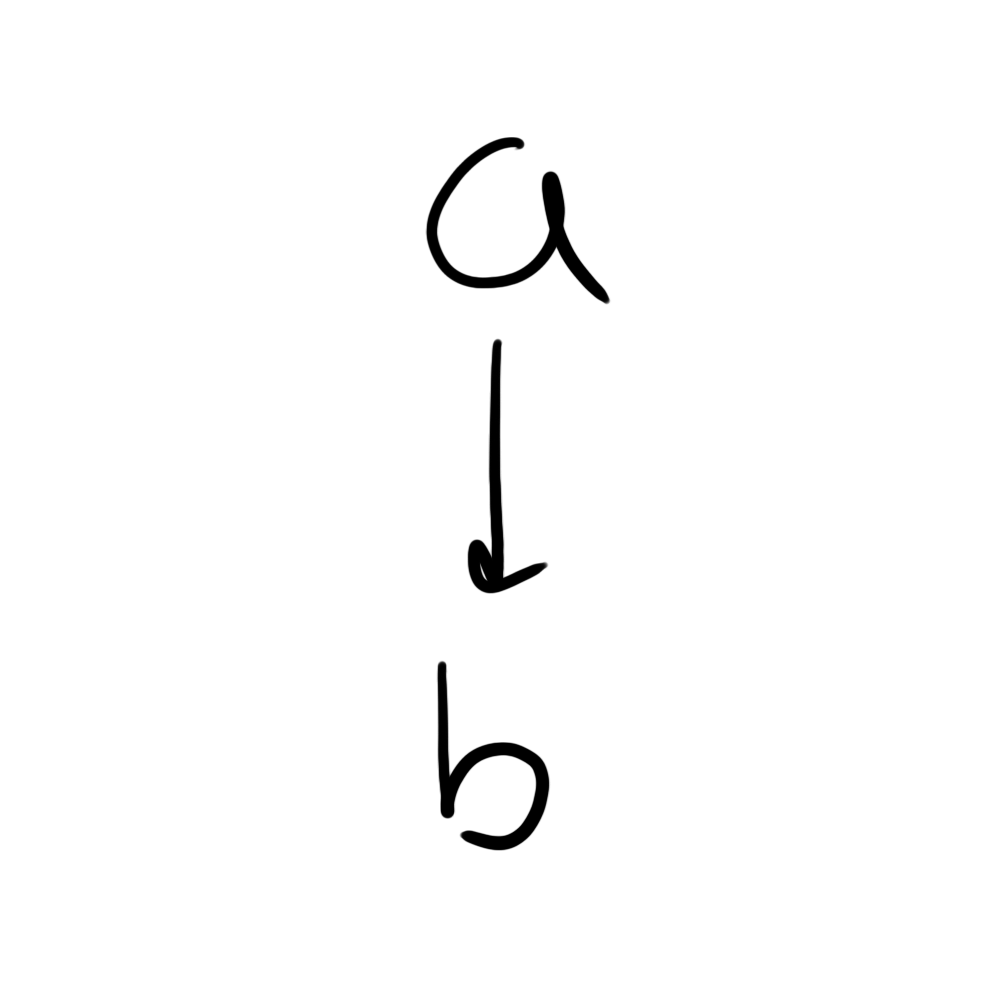
\includegraphics[scale=0.06]{gen11}
  \caption[] {
    \tabular[t]{@{}l@{}} ARS = (A, R) \\ A = \{a, b\} \\ R = \{(a, b)\}
    \endtabular}
\end{figure}

\begin{figure}[h!]
  \centering
  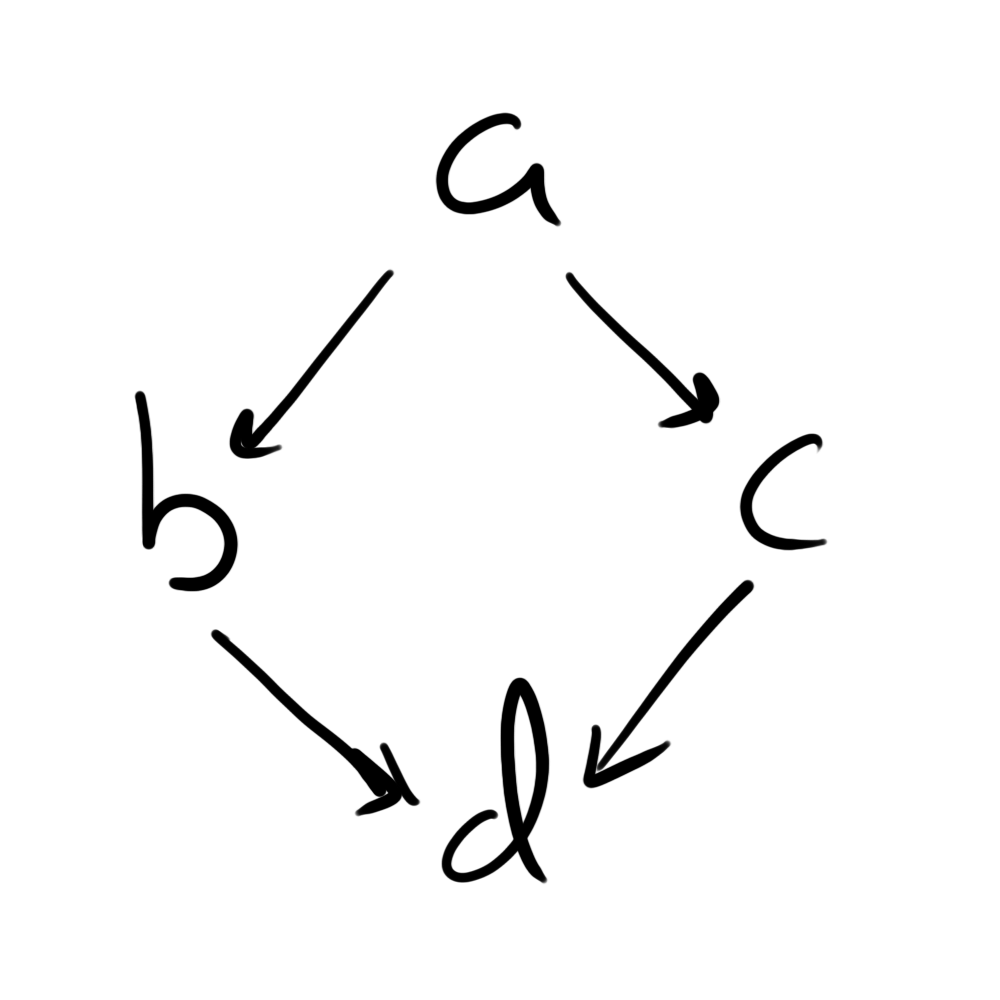
\includegraphics[scale=0.06]{gen12}
  \caption[] {
    \tabular[t]{@{}l@{}} ARS = (A, R) \\ \{a, b, c, d\} \\ R = \{(a, b), (a, c), (b, d), (c, d)\}
    \endtabular}
\end{figure}

\begin{figure}[h!]
  \centering
  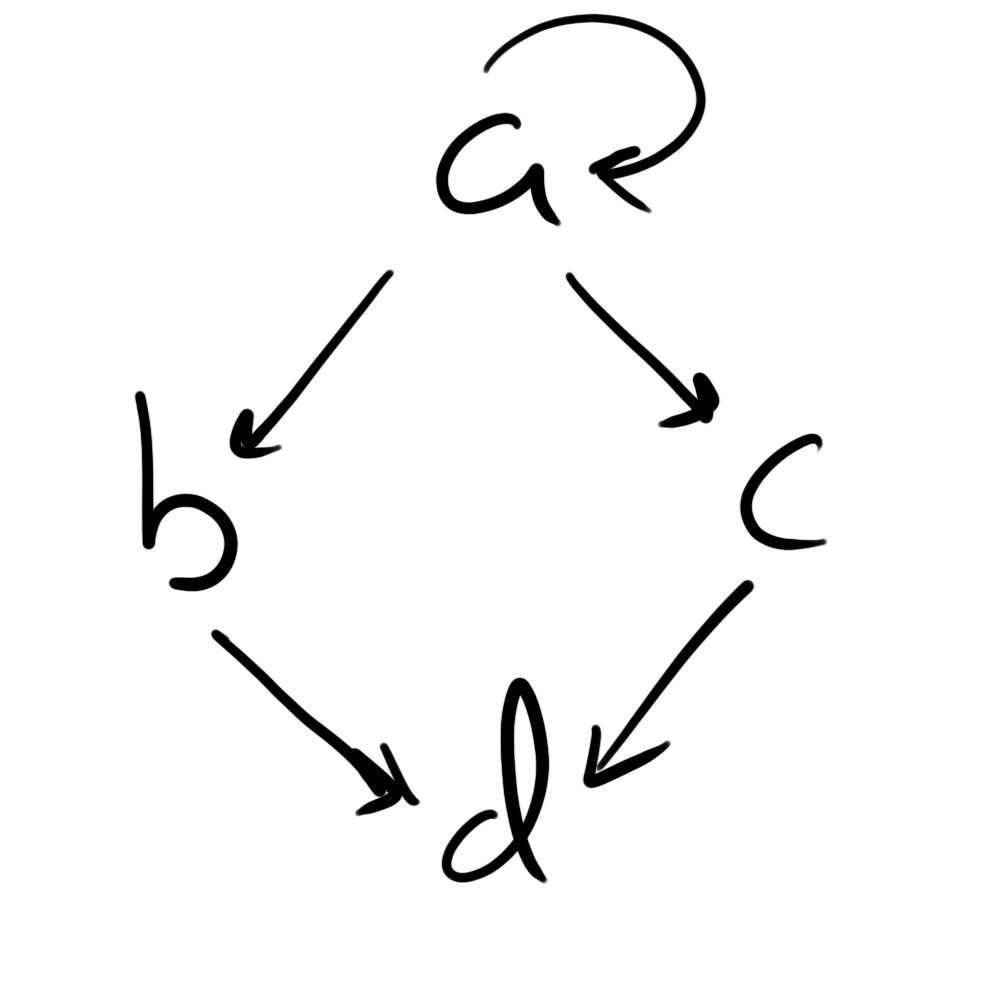
\includegraphics[scale=0.06]{gen13}
  \caption[] {
    \tabular[t]{@{}l@{}} ARS = (A, R) \\ A = \{a, b, c, d\} \\ R = \{(a, a), (a, b), (a, c), (b, d), (c, d)\}
    \endtabular}
\end{figure}

\medskip\noindent
As you can see, both of these examples reveal that each ARS leads to one UNF. Keep in mind that having a UNF does not imply that the ARS will be deterministic, since there can be a UNF in an ARS with loops. The third ARS above is an example of this. CONCLUDE


\subsubsection{Confluence}

\medskip\noindent
INTRODUCE AND ELABORATE ON CONFLUENCE. A simple way to think of this is that a confluent ARS has a peak for every valley. In the example below, a, b, and c represent the peak and b, c, and d represent the valley.

\begin{figure}[h!]
  \centering
  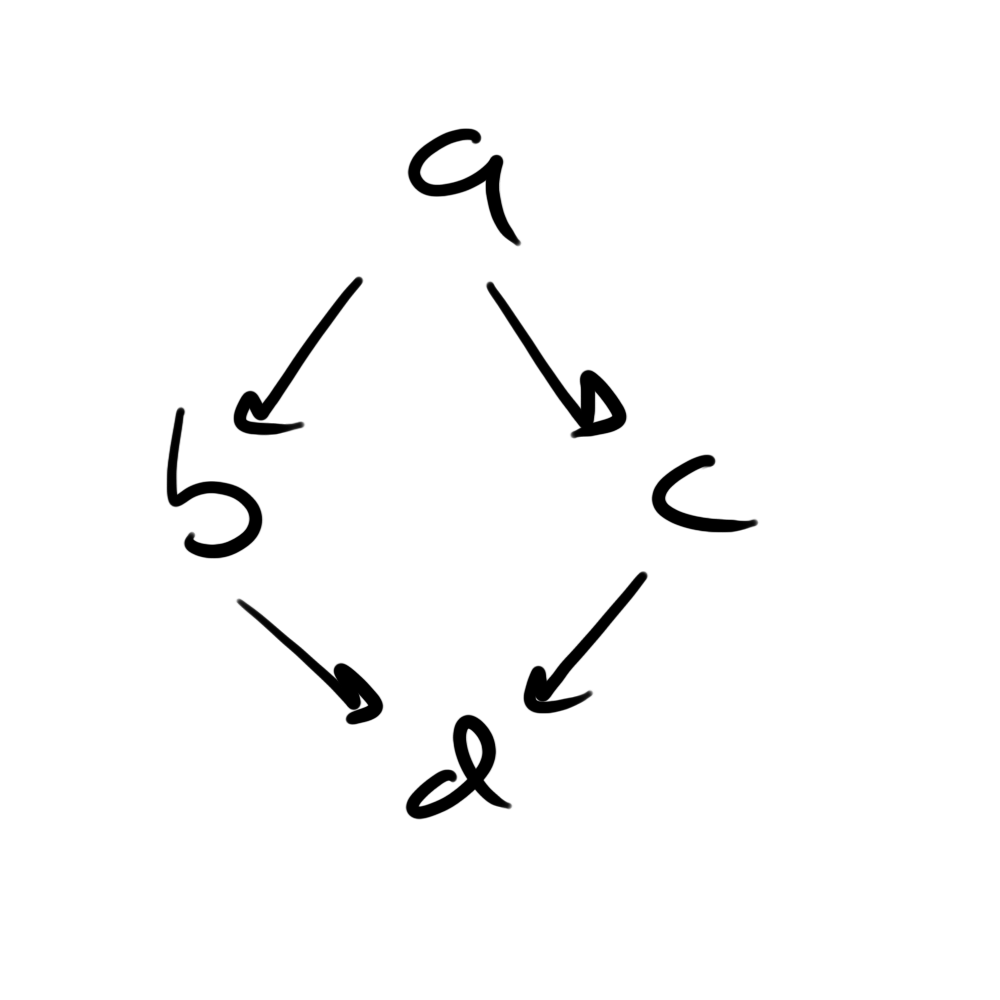
\includegraphics[scale=0.06]{gen14}
  \caption[] {
    \tabular[t]{@{}l@{}} ARS = (A, R) \\ A = \{a, b, c ,d\} \\ R = \{(a, b), (a, c), (b, d), (c, d)\}
    \endtabular}
\end{figure}

\medskip\noindent
Furthermore, if the ARS can take multiple routes to achieve the same result, then it is confluent. This can be seen in the confluent example above, since both routes (a $\rightarrow$ b $\rightarrow$ d) and (a $\rightarrow$ c $\rightarrow$ d) lead to the same result. Here are more examples of confluent ARS's.

\begin{figure}[h!]
  \centering
  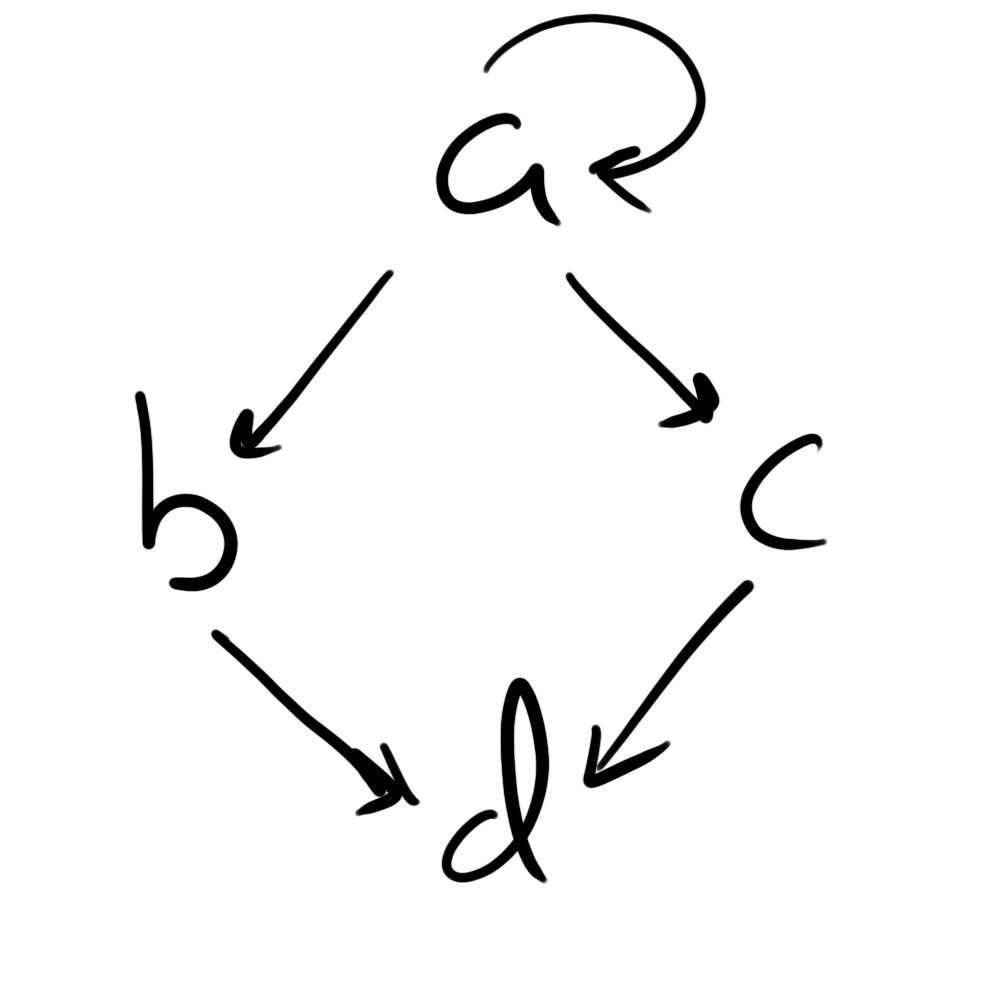
\includegraphics[scale=0.06]{gen15}
  \caption[] {
    \tabular[t]{@{}l@{}} ARS = (A, R) \\ A = \{a, b, c, d\} \\ R = \{(a, a), (a, b), (a, c), (b, d), (c, d)\}
    \endtabular}
\end{figure}

\begin{figure}[h!]
  \centering
  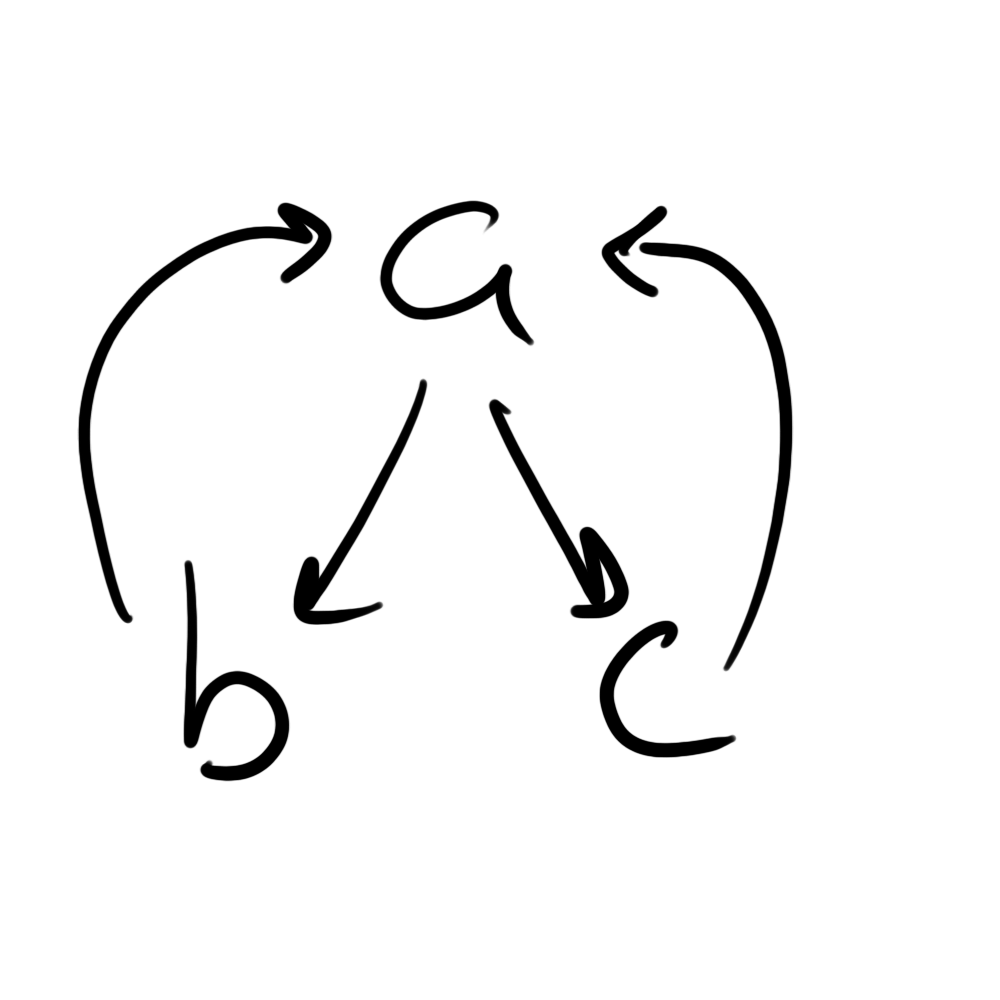
\includegraphics[scale=0.06]{gen16}
  \caption[] {
    \tabular[t]{@{}l@{}} ARS = (A, R) \\ A = \{a, b, c\} \\ R = \{(a, b), (a, c), (b, a), (c, a)\}
    \endtabular}
\end{figure}


\subsection{Relationships Between the Properties of Abstract Reduction Systems}

\medskip\noindent
By now, you may have begun to ponder the relationships between confluence, termination, and unique normal forms. More specifically, you may have suspected that not all combinations of these three properties are possible in ARS’s.

\medskip\noindent
Here is a chart with corresponding ARS's to help visualize these relationships. Keep in mind that other ARS's can apply to some of relationship combinations.

\begin{figure}[h!]
  \centering
  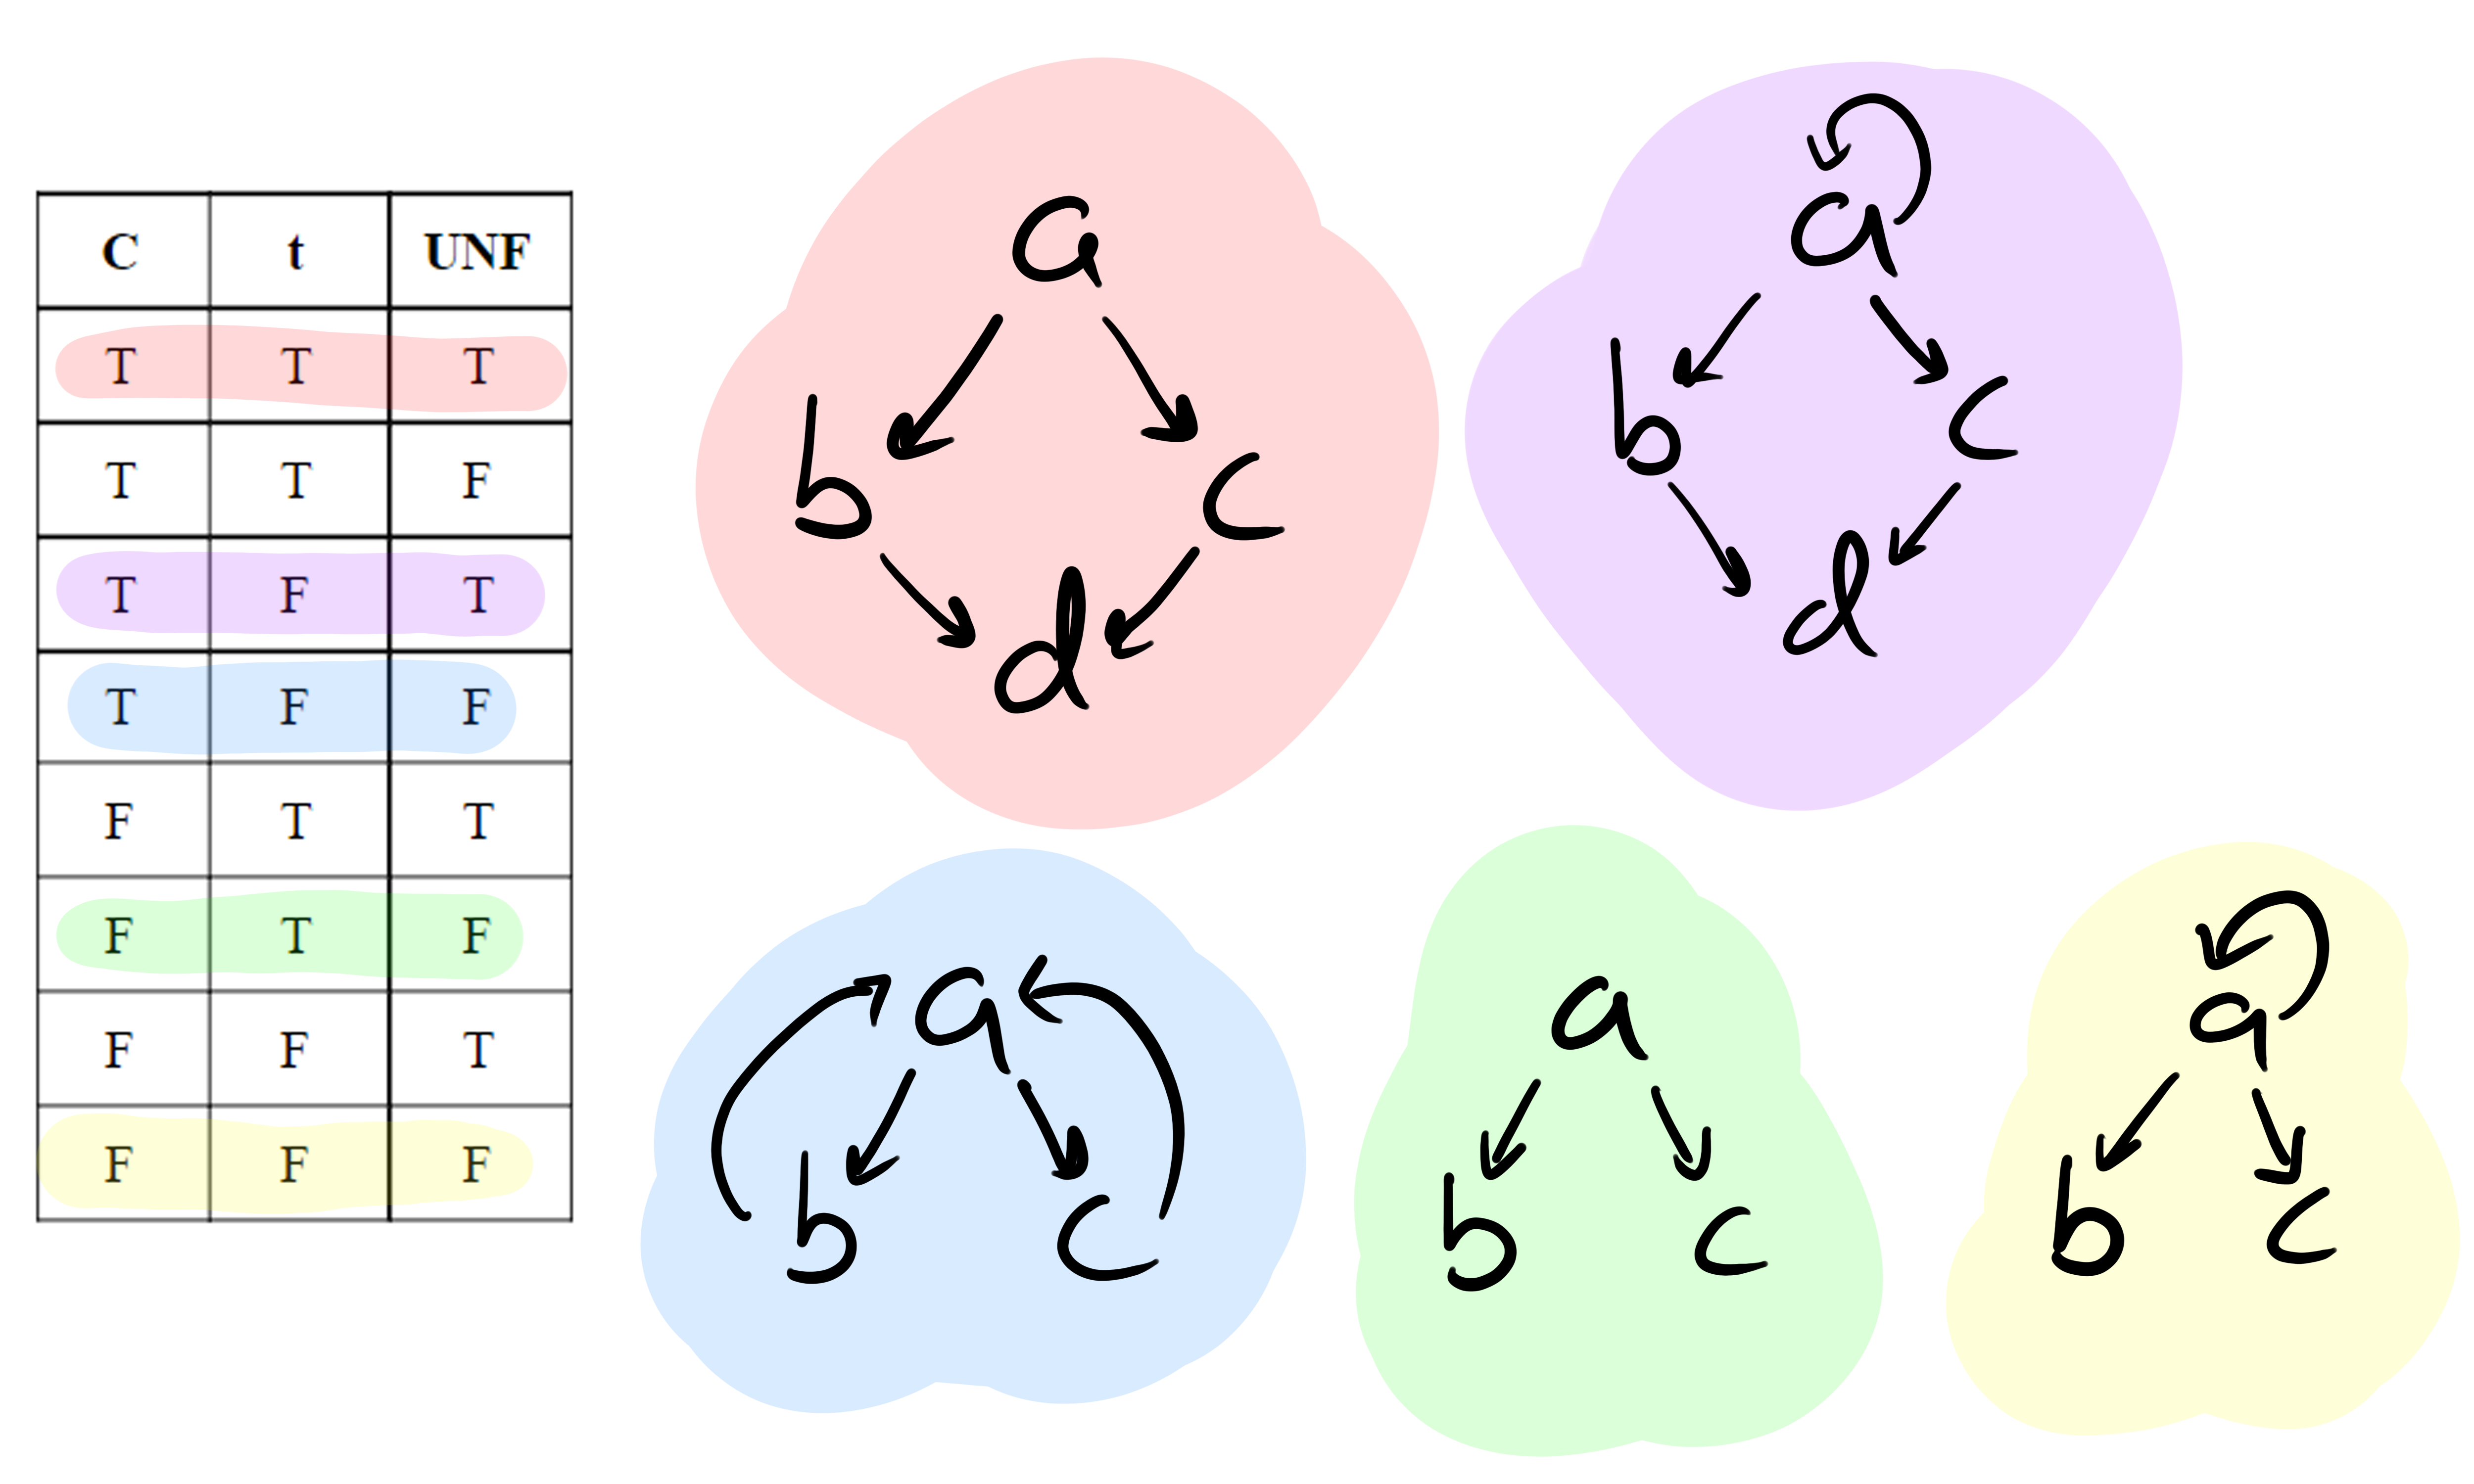
\includegraphics[scale=0.06]{arsComparisonGen}
\end{figure}

\medskip\noindent
Some of the cases that you may have encountered are that if an ARS is confluent and terminating, then it must have a UNF. Similarly, if an ARS is not confluent and then it cannot have a UNF. These relationships can be expressed in mathematical boolean notation:

$\neg$ (C $\land$ T $\land$ $\neg$ UNF)
$\neg$ ($\neg$ C $\land$ T $\land$ UNF)
$\neg$ ($\neg$ C $\land$ $\neg$ T $\land$ UNF)

\medskip\noindent
This can be simplified to:

SIMPLIFIED VERSION

\medskip\noindent
For reference, here is what the boolean notation would look like in C. MAKE SURE THIS IS CORRECT

\begin{lstlisting}[style=CStyle]
  !(C && T && !UNF)
  !(!C && T && UNF)
  !(!C && !T && UNF)
\end{lstlisting}

\medskip\noindent
This can be simplified too:

\begin{lstlisting}[style=CStyle]
  C && T == UNF
  !C && T == !UNF
  !C && !T == !UNF
\end{lstlisting}


\subsection{Visualizing Reflexive, Symmetric, and Transitive Traits}

\medskip\noindent
For this tutorial we will be using multiple ARS's denoted as (A, R). For each example, set (A) will be written twice as two separate columns. The purpose of this is to help visualize reflexivity, symmetry, and transitivity while providing an additional form of visualization. Comparing these two forms of visualization should make it easier to grasps these concepts. Keep in mind that the color blue will be used to express changes to the visualzations.

\subsubsection{Visualizing Reflexivity}

\medskip\noindent
Consider this ARS as both a two-column and traditional visualization.

\begin{figure}[h!]\
  \centering
  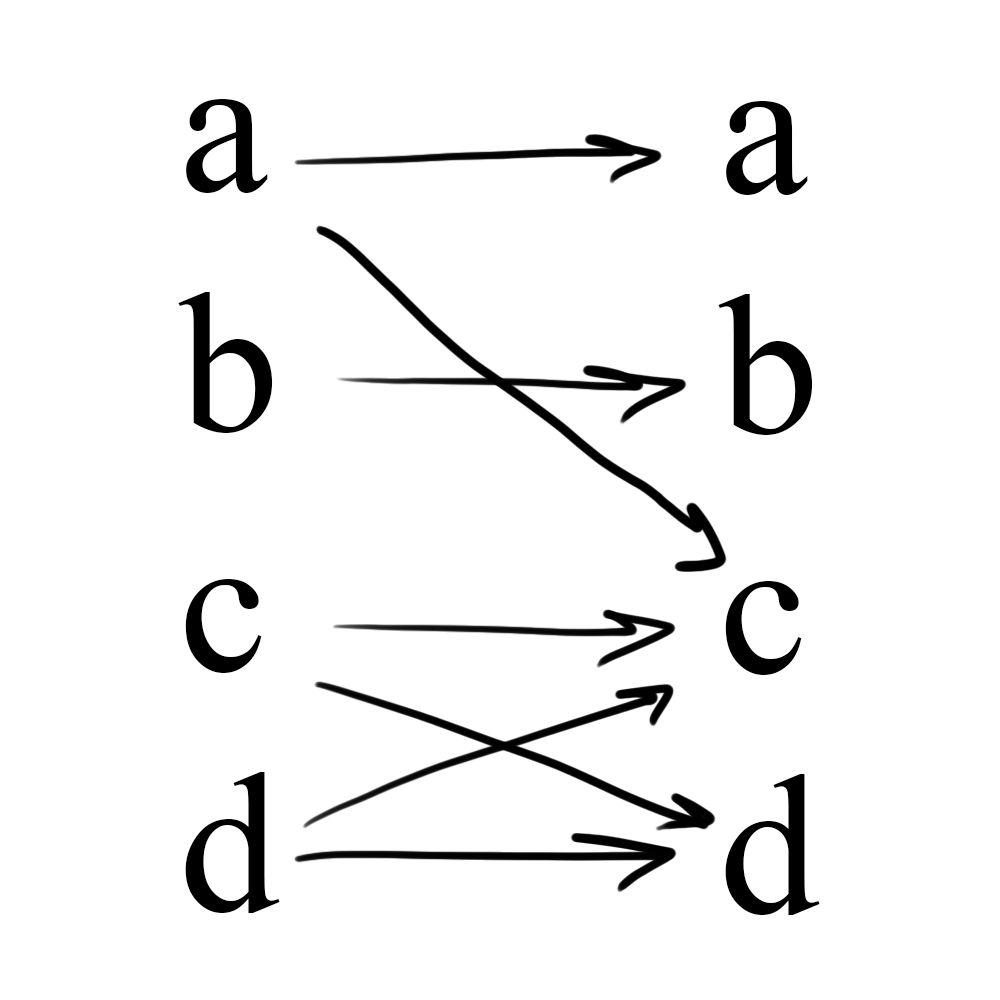
\includegraphics[scale=0.06]{s1}
  \caption[] {
    \tabular[t]{@{}l@{}} Two-column visualization of (A, R) \\ A = \{a, b, c ,d\} \\ R = \{(a, a), (a, c), (b, b), (c, c) (c, d), (d, d), (d, c)\}
    \endtabular}
\end{figure}

\begin{figure}[h!]
  \centering
  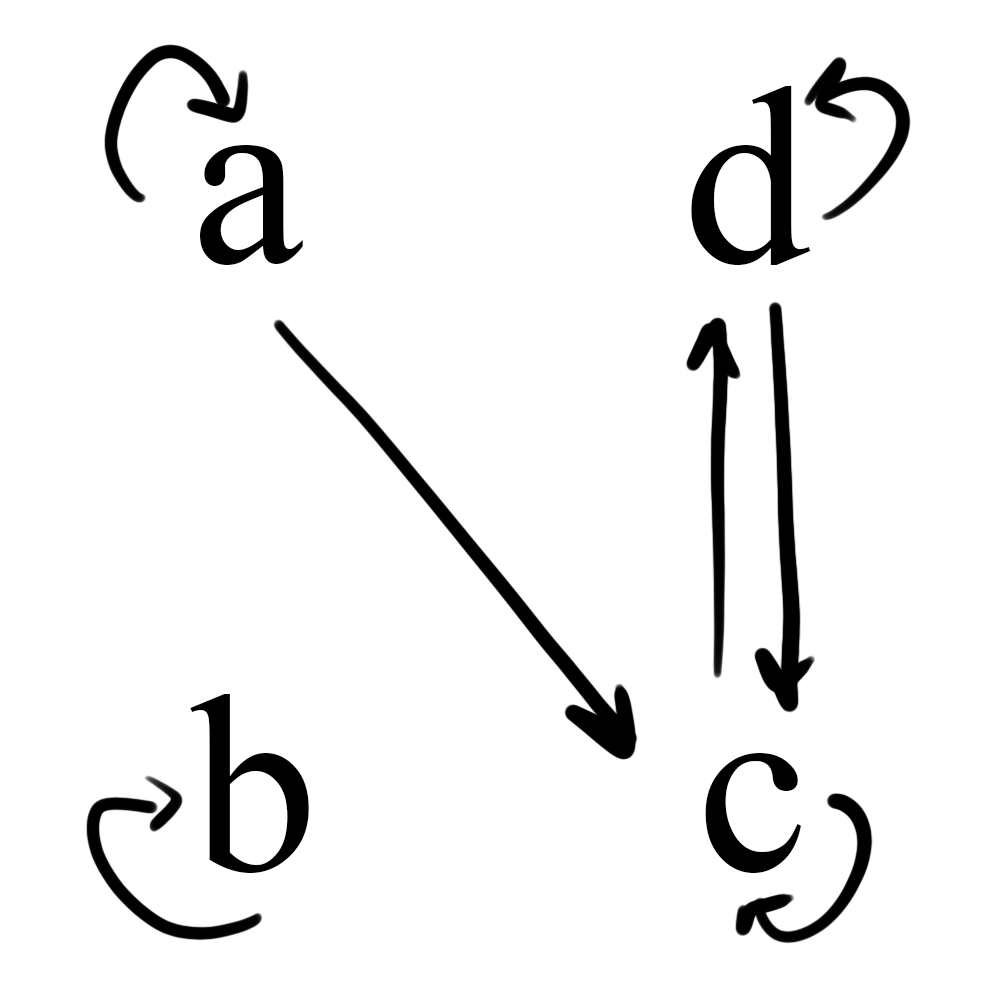
\includegraphics[scale=0.06]{v1}
  \caption[] {
    \tabular[t]{@{}l@{}} Traditional visualization
    \endtabular}
\end{figure}

\medskip\noindent
When an element points to itself, it is reflexive. In this example, every element is reflexive. Therefore, the entire set A is reflexive. However, if just one element did not point to itself, then the entire A could not be considered reflexive.

\subsubsection{Visualizing Symmetry}

\medskip\noindent
Taking a look at the same example from Figure 1, notice how the lower portion of the set A appears to be symmetric. This is because not only does c $\rightarrow$ d, but d $\rightarrow$ c too. Therefore there is symmetry between these two elements. However, since the entire set A is not symmetric, the set is considered asymmetrical. To make the set symmetric, we would have to make c $\rightarrow$ a.

\begin{figure}[h!]
  \centering
  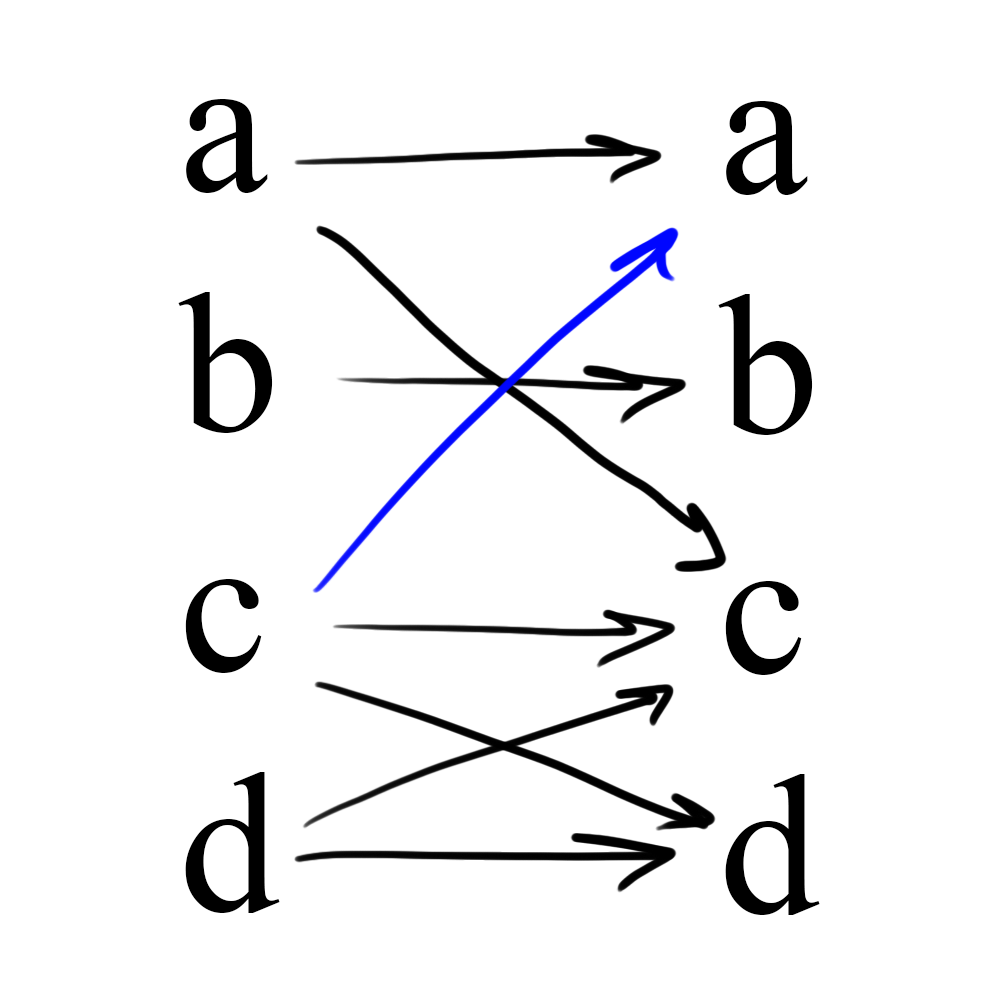
\includegraphics[scale=0.06]{s3}
  \caption[] {
    \tabular[t]{@{}l@{}} Symmetric two-column visualization of set A
    \endtabular}
\end{figure}

\begin{figure}[h!]
  \centering
  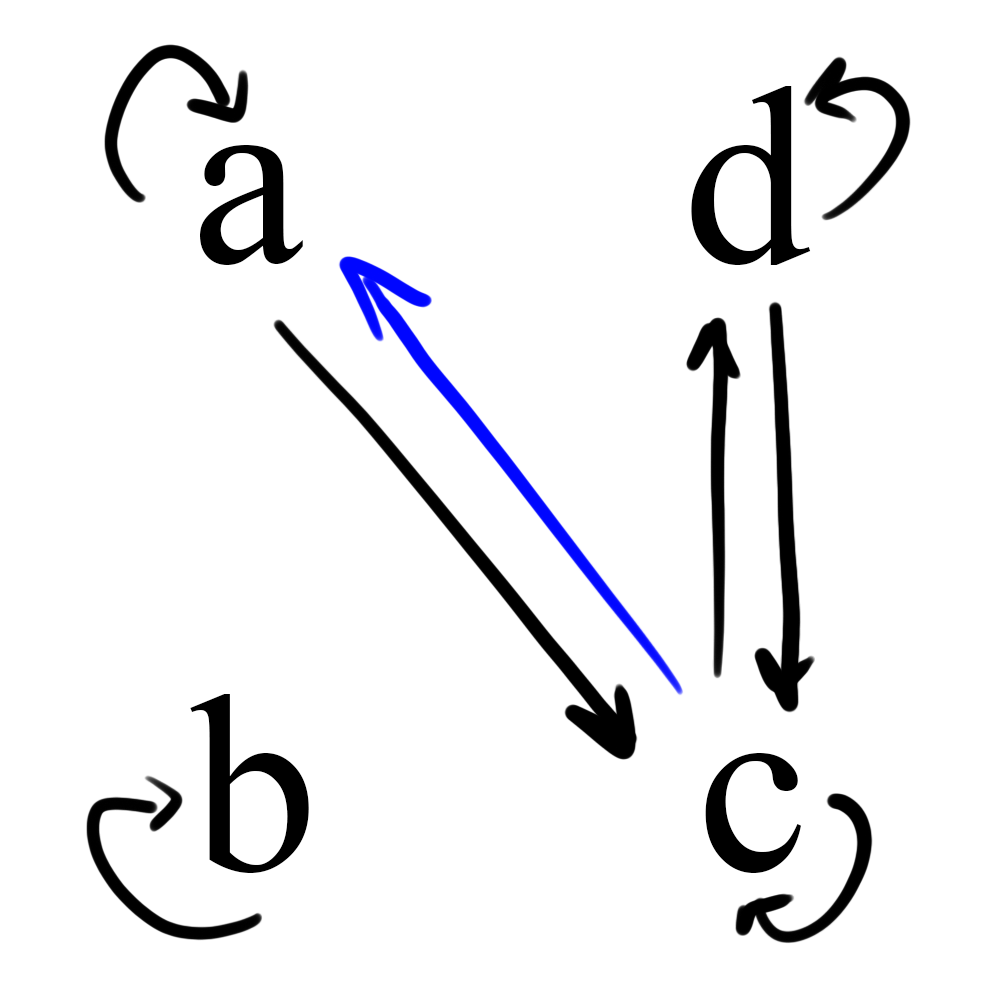
\includegraphics[scale=0.06]{v2}
  \caption[] {
    \tabular[t]{@{}l@{}} ARS = (A, R) \\ A = \{a, b, c ,d\} \\ R = \{(a, a), (a, c), (b, b), (c, c), (c, a), (c, d), (d, d), (d, c)\}
    \endtabular}
\end{figure}
    
\medskip\noindent
Notice how with symmetry, there are arrows going to and from (a, b) and (c, d). This can be rewritten with the proper notation using $\leftrightarrow$. The corrected ARS would look like:

\begin{figure}[h!]
  \centering
  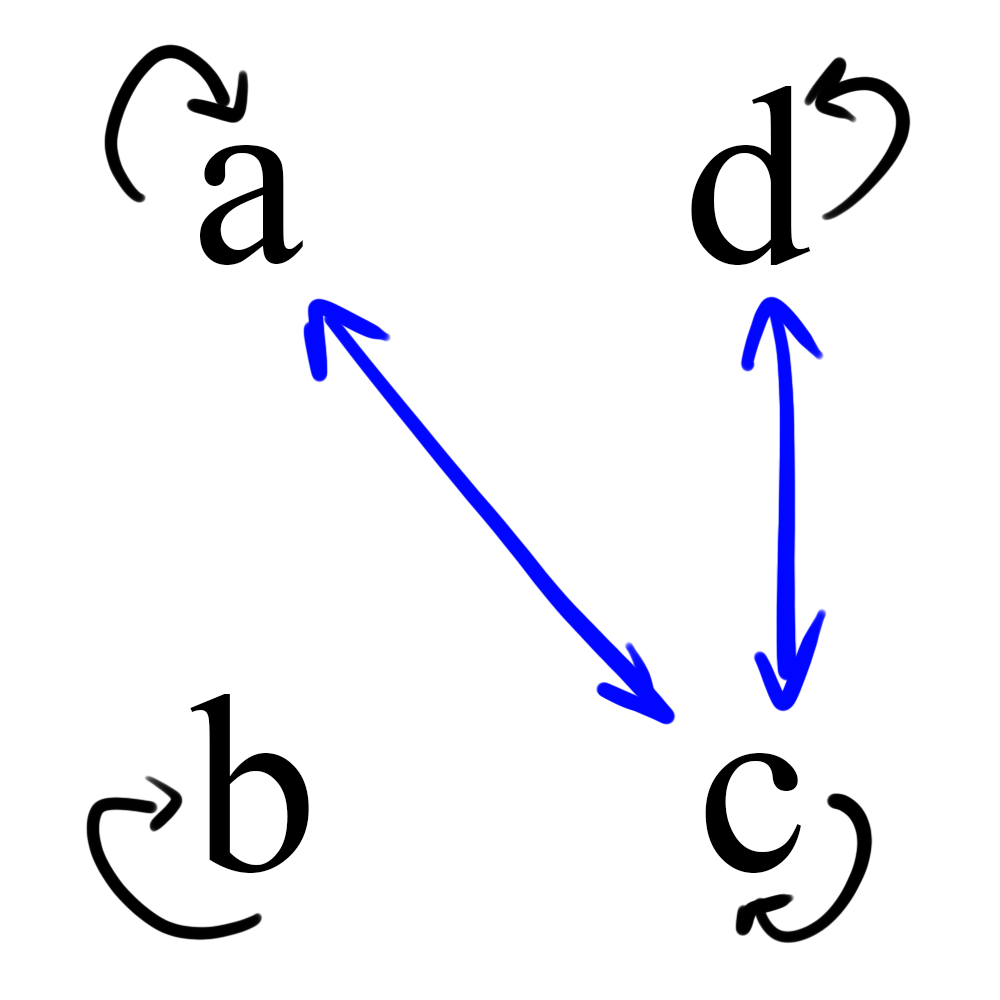
\includegraphics[scale=0.06]{v3}
  \caption[] {
    \tabular[t]{@{}l@{}} (A, R) with proper notation
    \endtabular}
\end{figure}

\medskip\noindent
With this way of visualizing the set, it is easy to see if it is symmetric as the drawing itself will almost be completely symmetrical. The only asymmetric quality of the drawing is that when an element is reflexive and is pointing to itself, it does not appear to point back. Keep in mind that it is also symmetric because it is simply pointing to itself.

\subsubsection{Visualizing Transitivity}
$\xrightarrow{\text{}}$

\medskip\noindent
INTRODUCE TRANSITIVITY HERE. To simplify the visualization, we will now work with this set:

\begin{figure}[h!]
  \centering
  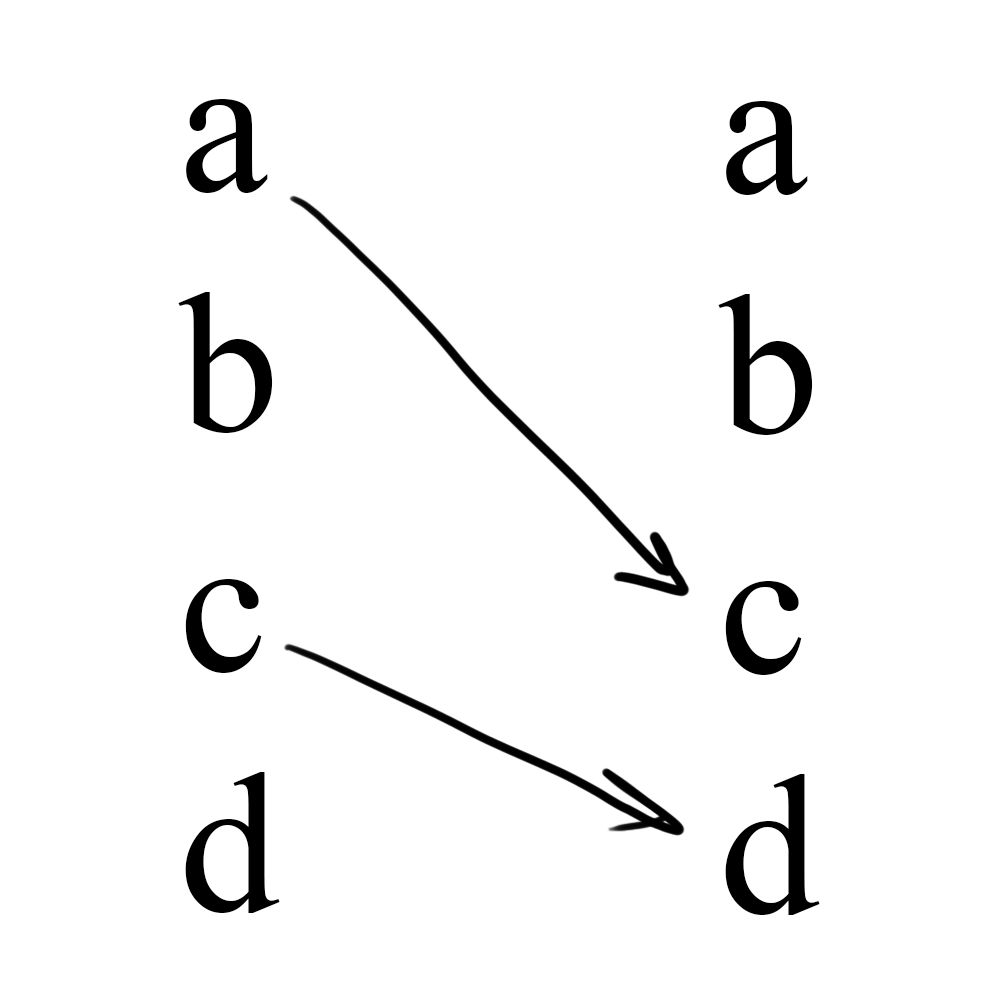
\includegraphics[scale=0.06]{s4}
  \caption[] {
    \tabular[t]{@{}l@{}} 2 column
    \endtabular}
\end{figure}

\begin{figure}[h!]
  \centering
  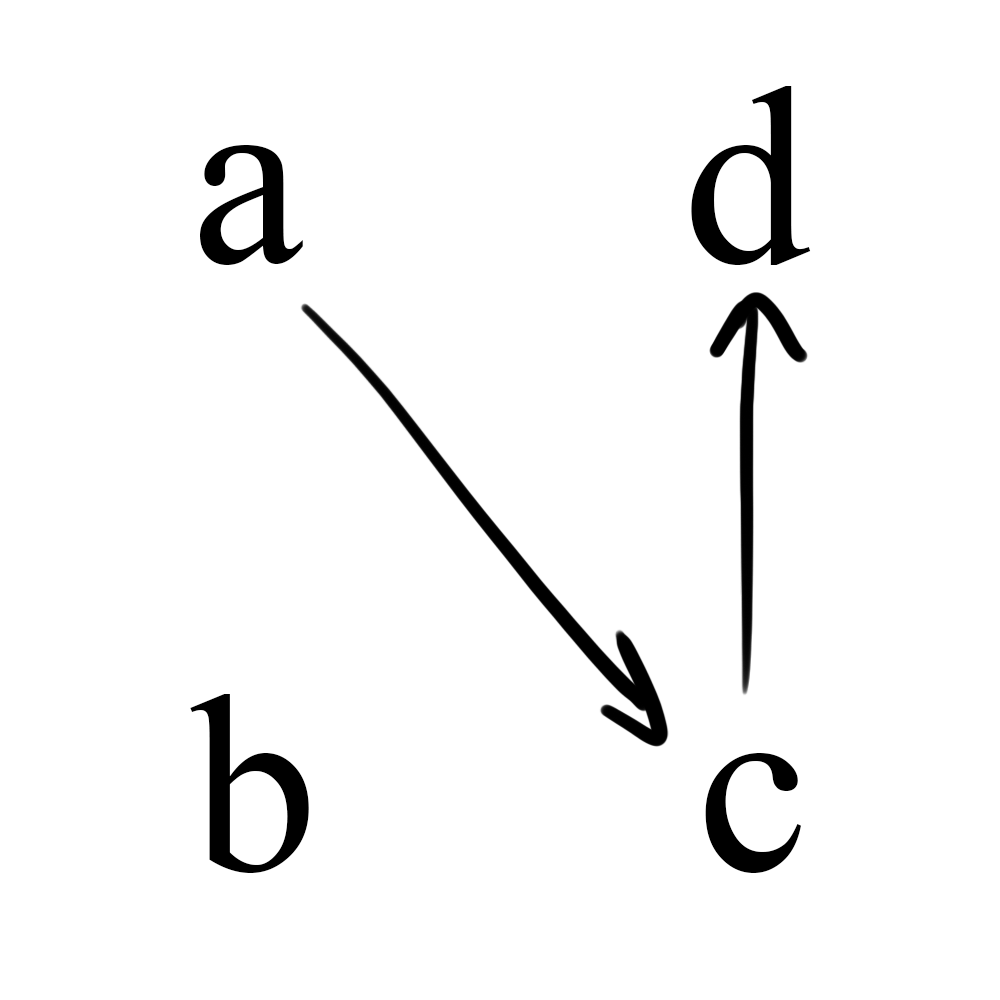
\includegraphics[scale=0.06]{v4}
  \caption[] {
    \tabular[t]{@{}l@{}} ARS = (A, R) \\ A = \{a, b, c ,d\} \\ R = \{(a, c), (c, d)\}
    \endtabular}
\end{figure}

\medskip\noindent
Notice how a $\rightarrow$ c and c $\rightarrow$ d. Shouldn’t that mean that there should be a shortcut from a → d? If this shortcut was added, and R was changed to R = \{(a, c), (a, d), (c, d)\} then (a, d) would be transitive. The notation for this would be $\xrightarrow{+}$. Here is the visualization of the separated set and the ARS:

\begin{figure}[h!]
  \centering
  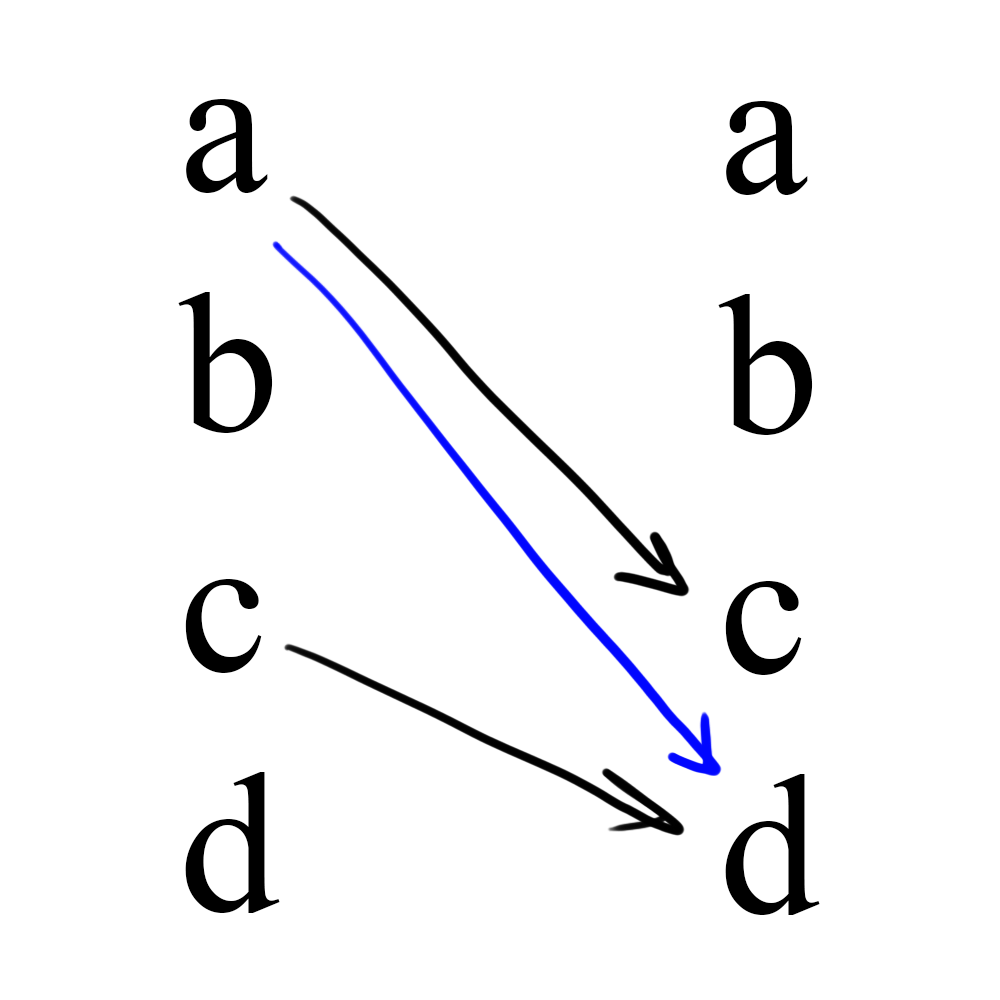
\includegraphics[scale=0.06]{s5}
  \caption[] {
    \tabular[t]{@{}l@{}} 2 column transitive
    \endtabular}
\end{figure}

\begin{figure}[h!]
  \centering
  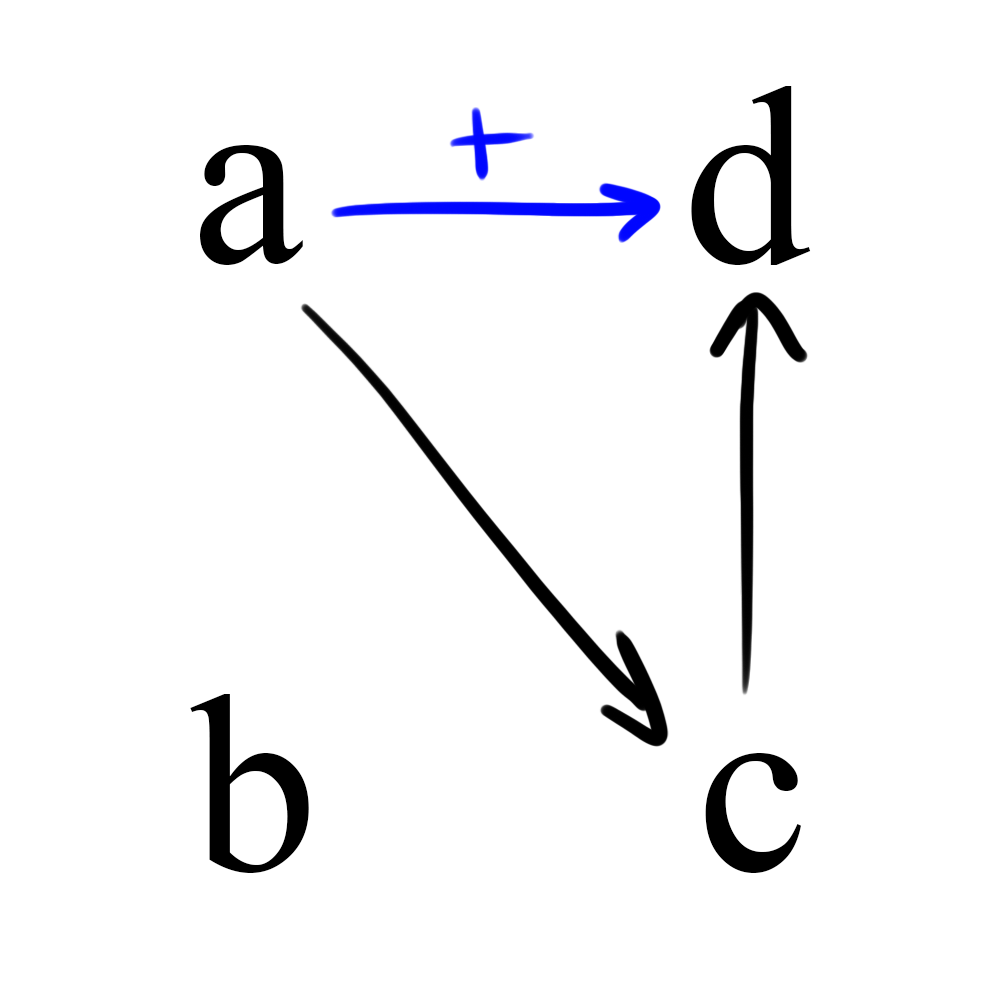
\includegraphics[scale=0.06]{v5}
  \caption[] {
    \tabular[t]{@{}l@{}} ARS = (A, R) \\ A = \{a, b, c ,d\} \\ R = \{(a, c), (a, d), (c, d)\}
    \endtabular}
\end{figure}

\medskip\noindent

\medskip\noindent

\medskip\noindent

\section{Project}

In this section you will describe a short project. It can either be in Haskell or of a theoretical nature,

\section{Conclusions}\label{conclusions}
At the beginning of this report, we explored Haskell by working with small examples and differentiating both syntax and theoretical difference between imperative C code and functional Haskell Code. This will be more elaborate when the rest of the report is completed. CONCLUDE THEORY.

\begin{thebibliography}{99}

\bibitem[PL]{PL} \href{https://github.com/alexhkurz/programming-languages-2021/blob/main/README.md}{Programming Languages 2021}, Chapman University, 2021.

\bibitem[HI]{HI} \href{https://www.youtube.com/watch?v=Vgu82wiiZ90&list=PLe7Ei6viL6jGp1Rfu0dil1JH1SHk9bgDV&index=1}{Haskell for Imperative Programmers}, Philipp Hagenlocher, 2020.

\bibitem[HI]{HI} \href{https://www.youtube.com/watch?v=Vgu82wiiZ90&list=PLe7Ei6viL6jGp1Rfu0dil1JH1SHk9bgDV&index=1}{Haskell for Imperative Programmers}, Philipp Hagenlocher, 2020.

\bibitem[HR]{HR} \href{https://en.wikibooks.org/wiki/Haskell/Recursion}{Haskell/Recursion}, WikiBooks, 2020.

\bibitem[PM]{PM} \href{https://stackoverflow.com/questions/2225774/haskell-pattern-matching-what-is-it}{Pattern Matching}, Stack Overflow, 2010.

\bibitem[LE]{LE} \href{https://wiki.haskell.org/Lazy_evaluation}{Lazy Evaluation}, Haskell Wiki, 2021.

\bibitem[ID]{ID} \href{https://learntocodetogether.com/imperative-vs-declarative-programming/}{Imperative vs. Declarative Programming}, Learn To Code Together, 2019.

\bibitem[HP]{HP} \href{https://wiki.haskell.org/Pure}{Pure}, Haskell Wiki, 2021.

\bibitem[GD]{GD} \href{https://docs.google.com/document/d/1e3_r3ifWnFcBaKs21iCF-OhED9x0NcDK59SA80lQjXY/edit?usp=sharing}{Google Doc}, I will cite the sources linked at the end of this doc.

\end{thebibliography}

\end{document}